\documentclass[journal]{vgtc}                % final (journal style)
%\documentclass[review,journal]{vgtc}         % review (journal style)
%\documentclass[widereview]{vgtc}             % wide-spaced review
%\documentclass[preprint,journal]{vgtc}       % preprint (journal style)

%% Uncomment one of the lines above depending on where your paper is
%% in the conference process. ``review'' and ``widereview'' are for review
%% submission, ``preprint'' is for pre-publication, and the final version
%% doesn't use a specific qualifier.

%% Please use one of the ``review'' options in combination with the
%% assigned online id (see below) ONLY if your paper uses a double blind
%% review process. Some conferences, like IEEE Vis and InfoVis, have NOT
%% in the past.

%% Please note that the use of figures other than the optional teaser is not permitted on the first page
%% of the journal version.  Figures should begin on the second page and be
%% in CMYK or Grey scale format, otherwise, colour shifting may occur
%% during the printing process.  Papers submitted with figures other than the optional teaser on the
%% first page will be refused. Also, the teaser figure should only have the
%% width of the abstract as the template enforces it.

%% These few lines make a distinction between latex and pdflatex calls and they
%% bring in essential packages for graphics and font handling.
%% Note that due to the \DeclareGraphicsExtensions{} call it is no longer necessary
%% to provide the the path and extension of a graphics file:
%% 
\includegraphics{diamondrule} is completely sufficient.
%%
\ifpdf%                                % if we use pdflatex
  \pdfoutput=1\relax                   % create PDFs from pdfLaTeX
  \pdfcompresslevel=9                  % PDF Compression
  \pdfoptionpdfminorversion=7          % create PDF 1.7
  \ExecuteOptions{pdftex}
  \usepackage{graphicx}                % allow us to embed graphics files
  \DeclareGraphicsExtensions{.pdf,.png,.jpg,.jpeg} % for pdflatex we expect .pdf, .png, or .jpg files
\else%                                 % else we use pure latex
  \ExecuteOptions{dvips}
  \usepackage{graphicx}                % allow us to embed graphics files
  \DeclareGraphicsExtensions{.eps}     % for pure latex we expect eps files
\fi%

%% it is recomended to use ``\autoref{sec:bla}'' instead of ``Fig.~\ref{sec:bla}''
\graphicspath{{figures/}{pictures/}{images/}{./}} % where to search for the images

\usepackage[utf8]{inputenc}
\usepackage{microtype}                 % use micro-typography (slightly more compact, better to read)
\PassOptionsToPackage{warn}{textcomp}  % to address font issues with \textrightarrow
\usepackage{textcomp}                  % use better special symbols
\usepackage{mathptmx}                  % use matching math font
\usepackage{times}                     % we use Times as the main font
\renewcommand*\ttdefault{txtt}         % a nicer typewriter font
\usepackage{cite}                      % needed to automatically sort the references
%\usepackage{color}
\usepackage{xcolor} % Some more colors not defined in "color" package
% \usepackage{tabu}                      % only used for the table example
% \usepackage{booktabs}                  % only used for the table example
\usepackage{todonotes}
\usepackage[draft]{hyperref} % Weird error occurs without this.
\usepackage{graphicx}
\usepackage{caption}
\usepackage{subcaption}
\usepackage[]{algorithm2e}
\usepackage{textgreek}
\usepackage{tikz, pgfplots}

\newcommand{\kallecomment}[1]{\textbf{[-Kalle-~}
    \textcolor{orange}{#1}
    \textbf{~]}}

\newcommand{\emilcomment}[1]{\textbf{[-Emil-~}
    \textcolor{red}{#1}
    \textbf{~]}}

\newcommand{\alexcomment}[1]{\textbf{[-Alex-~}
    \textcolor{magenta}{#1}
    \textbf{~]}}

\newcommand{\anderscomment}[1]{\textbf{[-Anders-~}
    \textcolor{cyan}{#1}
    \textbf{~]}}
\newcommand{\plgrem}[1]{\textcolor{blue}{~\textbf{!!}~}}

\newcommand{\fig}[1]{Figure~\ref{fig:#1}}

\newcommand{\etal}{\emph{et~al.}}

\setlength{\fboxsep}{0pt}


%% We encourage the use of mathptmx for consistent usage of times font
%% throughout the proceedings. However, if you encounter conflicts
%% with other math-related packages, you may want to disable it.

%% In preprint mode you may define your own headline.
%\preprinttext{To appear in IEEE Transactions on Visualization and Computer Graphics.}

%% If you are submitting a paper to a conference for review with a double
%% blind reviewing process, please replace the value ``0'' below with your
%% OnlineID. Otherwise, you may safely leave it at ``0''.
\onlineid{120}

%% declare the category of your paper, only shown in review mode
\vgtccategory{Research}
%% please declare the paper type of your paper to help reviewers, only shown in review mode
%% choices:
%% * algorithm/technique
%% * application/design study
%% * evaluation
%% * system
%% * theory/model
\vgtcpapertype{application}

%% Paper title.

\title{Globe Browsing: Contextualized Spatio-Temporal \\
Planetary Surface Visualization}

%% This is how authors are specified in the journal style

%% indicate IEEE Member or Student Member in form indicated below
\author{Submission \#120 \\
\\
Karl Bladin, Emil Axelsson, Erik Broberg, Carter Emmart, Patric Ljung, \\ Alexander Bock and Anders Ynnerman, \textit{Associate Member, IEEE}}

\authorfooter{
%% insert punctuation at end of each item
\item
Karl Bladin, Emil Axelsson, Patric Ljung, Anders Ynnerman and Erik Broberg are with Link\"oping University.
E-mail: \{ karl.bladin, emil.axelsson, patric.ljung, anders.ynnerman \} @liu.se, eribr049@student.liu.se
\item
Carter Emmart is with American Museum of Natural History. E-mail: carter@amnh.org.
\item
Alexander Bock is with New York University and Link\"oping University. E-mail: alexander.bock@nyu.edu
}

%other entries to be set up for journal
\shortauthortitle{Bladin \MakeLowercase{\textit{et al.}}: Globe Browsing}

%% Abstract section.
\abstract{%
% Submitted version of the abstract
%We present work on tailoring and integration of multiple data processing and visualization methods to interactively contextualize geospatial data of celestial bodies for use in public science dissemination and communication between domain scientists.
%Results of planetary mapping is often shared openly for use in scientific research and mission planning.
%However, this data is, in its raw format, not accessible to non-experts, as it is difficult to grasp the context of the data and the intricate acquisition process.
%As our approach is full interactive and handles dynamic data sources, we are significantly shortening the time between discovery and dissemination of data and results.
%We describe the image acquisition, required pre-processing steps to derive a 2.5D terrain, and a chunked level-of-detail, out-of-core rendering approach to enable interactive exploration of global maps as well as high-resolution digital terrain models.
%One interesting case is Mars as extensive amount of map data is available from various missions.
%A second case is dynamical processes, such as weather conditions on Earth that require spatio-temporal datasets.
%In addition to visualizing the scientific results, we also present ongoing data acquisition, exemplified in the Pluto flyby of the New Horizons spacecraft.
%Our work has been implemented in the OpenSpace software, which enables interactive presentations in a range of environments such as immersive dome theaters and virtual reality headsets.
%
Results of planetary mapping is often shared openly for use in scientific research and mission planning.
However, in its raw format, the data is not accessible to non-experts due to the difficulty in grasping the context of the data and the intricate acquisition process.
We present work on tailoring and integration of multiple data processing and visualization methods to interactively contextualize geospatial surface data of celestial bodies for use in science communication.
As our approach handles dynamic data sources, streamed from on-line repositories, we are significantly shortening the time between discovery and dissemination of data and results.
We describe the image acquisition pipeline, pre-processing steps to derive a 2.5D terrain, and a chunked level-of-detail, out-of-core rendering approach to enable interactive exploration of global maps and high-resolution digital terrain models.
The results are demonstrated for three different celestial bodies.
The first case is high-resolution map data on the surface of Mars.
A second case is showing dynamical processes, such as high-resolution and concurrent weather conditions on Earth that require spatio-temporal datasets.
As a final example we use data from the New Horizons spacecraft which acquired data during a single flyby of Pluto.
We visualize the acquisition process as well as the resulting surface data.  
Our work has been implemented in the OpenSpace software, which enables interactive presentations in a range of environments such as immersive dome theaters and virtual reality headsets.

%
% In addition, the application supports temporal datasets, where available, in order to visualize a celestial body's dynamic processes, such as weather conditions on Earth.
% Furthermore, we interactively play back in-situ visualizations of the process for data acquisition.
%
%
%We present an application where scientific mapping data of celestial bodies is contextualized in space and time to enrich the experience in public dissemination as well as to support communication between scientists.
%In our system various types of datasets and visualization techniques are combined.
%A chunked level-of-detail approach is used to enable interactive exploration of global maps as well as local high-resolution digital terrain models with textures and height information.
%This is particularly interesting for Mars thanks to the extensive amount of map data gathered by the various missions to this planet.
%Using time varying datasets, we visualize the dynamics of a celestial body, such as weather conditions on Earth.
%Furthermore, we interactively play back in-situ visualizations of the process for data acquisition.
%
%Our work has been implemented in the open source software OpenSpace, which enables interactive presentations in immersive environments like dome theaters and virtual reality headsets.
%
%
%
%
%
%The mapping of the planets and moons within our solar system is carried out by space organizations such as NASA and ESA.
%Image data are collected by cameras on satellites and spacecraft, and used in scientific research and in planning of future space missions.
%Despite the fact that NASA shares a lot of its image data openly, it seldom reaches the general public.
%
%A lot of research has been done in terms of visualizing planetary data using terrain rendering. Current technology relies on techniques such as out-of-core, and dynamic level-of-detail rendering, multi threaded data acquisition and consideration of precision limitations.
%
%These systems are often either specialized for researchers where accuracy is the main concern, or for games, where the user experience plays a major role.
%
%We present an application for visualizing the same data that space scientists analyze in the context of a virtual environment representing the space that we are exploring.
%Given the contextualization that the real space provides, we can model the solar system using positional data for modelling the planets' orbits together with the space probes that explores them.
%In a time varying visualizations we can show the dynamics of a planetary surface as well as the data collection process itself.
%
%The main focus of this paper is to describe the combination of different datasets gathered for mapping out planets' surface features. 
% particularly Mars due to the extensive amount of map data gathered by the various missions on this planet.
%
%Our rendering system combines various resolutions of local and global map datasets and presents them together in their real context.
%Using the Geospatial Data Abstraction Library (GDAL), we can preprocess images to match the most common cylindrical projection format used for globe rendering.
%A chunked level-of-detail approach is used for rendering tiles which are height mapped on the fly.
%This allows for a versatile globe renderer which can easily load new datasets without requiring preprocessing by the rendering software.
%
%We can use the same data that scientists use in their research for public dissemination and present it, bundled and contextualized, using immersive rendering systems.
%Our software, OpenSpace, is an open source project with the goal of bringing space science to the general public.
%
%
% The mapping of the planets and moons within our solar system is carried out by space organizations such as NASA and
% ESA. Image data are collected by instruments on satellites and spacecraft, and subsequently used in scientific research and mission
% planning. While map data from space missions are often shared openly, it can be difficult for non-experts to comprehend the context of
% the data and understand the acquisition process.
% We present an application where scientific mapping data of celestial bodies is contextualized in space and time to enrich the experience
% in public dissemination as well as to support communication between scientists. In our system various types of datasets and
% visualization techniques are combined; A chunked level-of-detail approach is used to enable interactive exploration of global maps as
% well as local high-resolution digital terrain models with textures and height information. This is particularly interesting for Mars thanks
% to the extensive amount of map data gathered by the various missions to this planet. Using time varying datasets, we visualize the
% dynamics of a celestial body, such as weather conditions on Earth. Furthermore, we interactively play back in-situ visualizations of the
% process for data acquisition.
% Our work has been implemented in the open source software OpenSpace that enables interactive presentations in immersive
% environments like dome theaters and virtual reality headsets.
%
%
} % end of abstract

%% Keywords that describe your work. Will show as 'Index Terms' in journal
%% please capitalize first letter and insert punctuation after last keyword
\keywords{Astronomical visualization, globe rendering, public dissemination, science communication, space mission visualization }

%% ACM Computing Classification System (CCS). 
%% See <http://www.acm.org/class/1998/> for details.
%% The ``\CCScat'' command takes four arguments.

\CCScatlist{ % not used in journal version
 \CCScat{K.6.1}{Management of Computing and Information Systems}%
{Project and People Management}{Life Cycle};
 \CCScat{K.7.m}{The Computing Profession}{Miscellaneous}{Ethics}
}

%% Uncomment below to include a teaser figure.
\teaser{
  \centering
  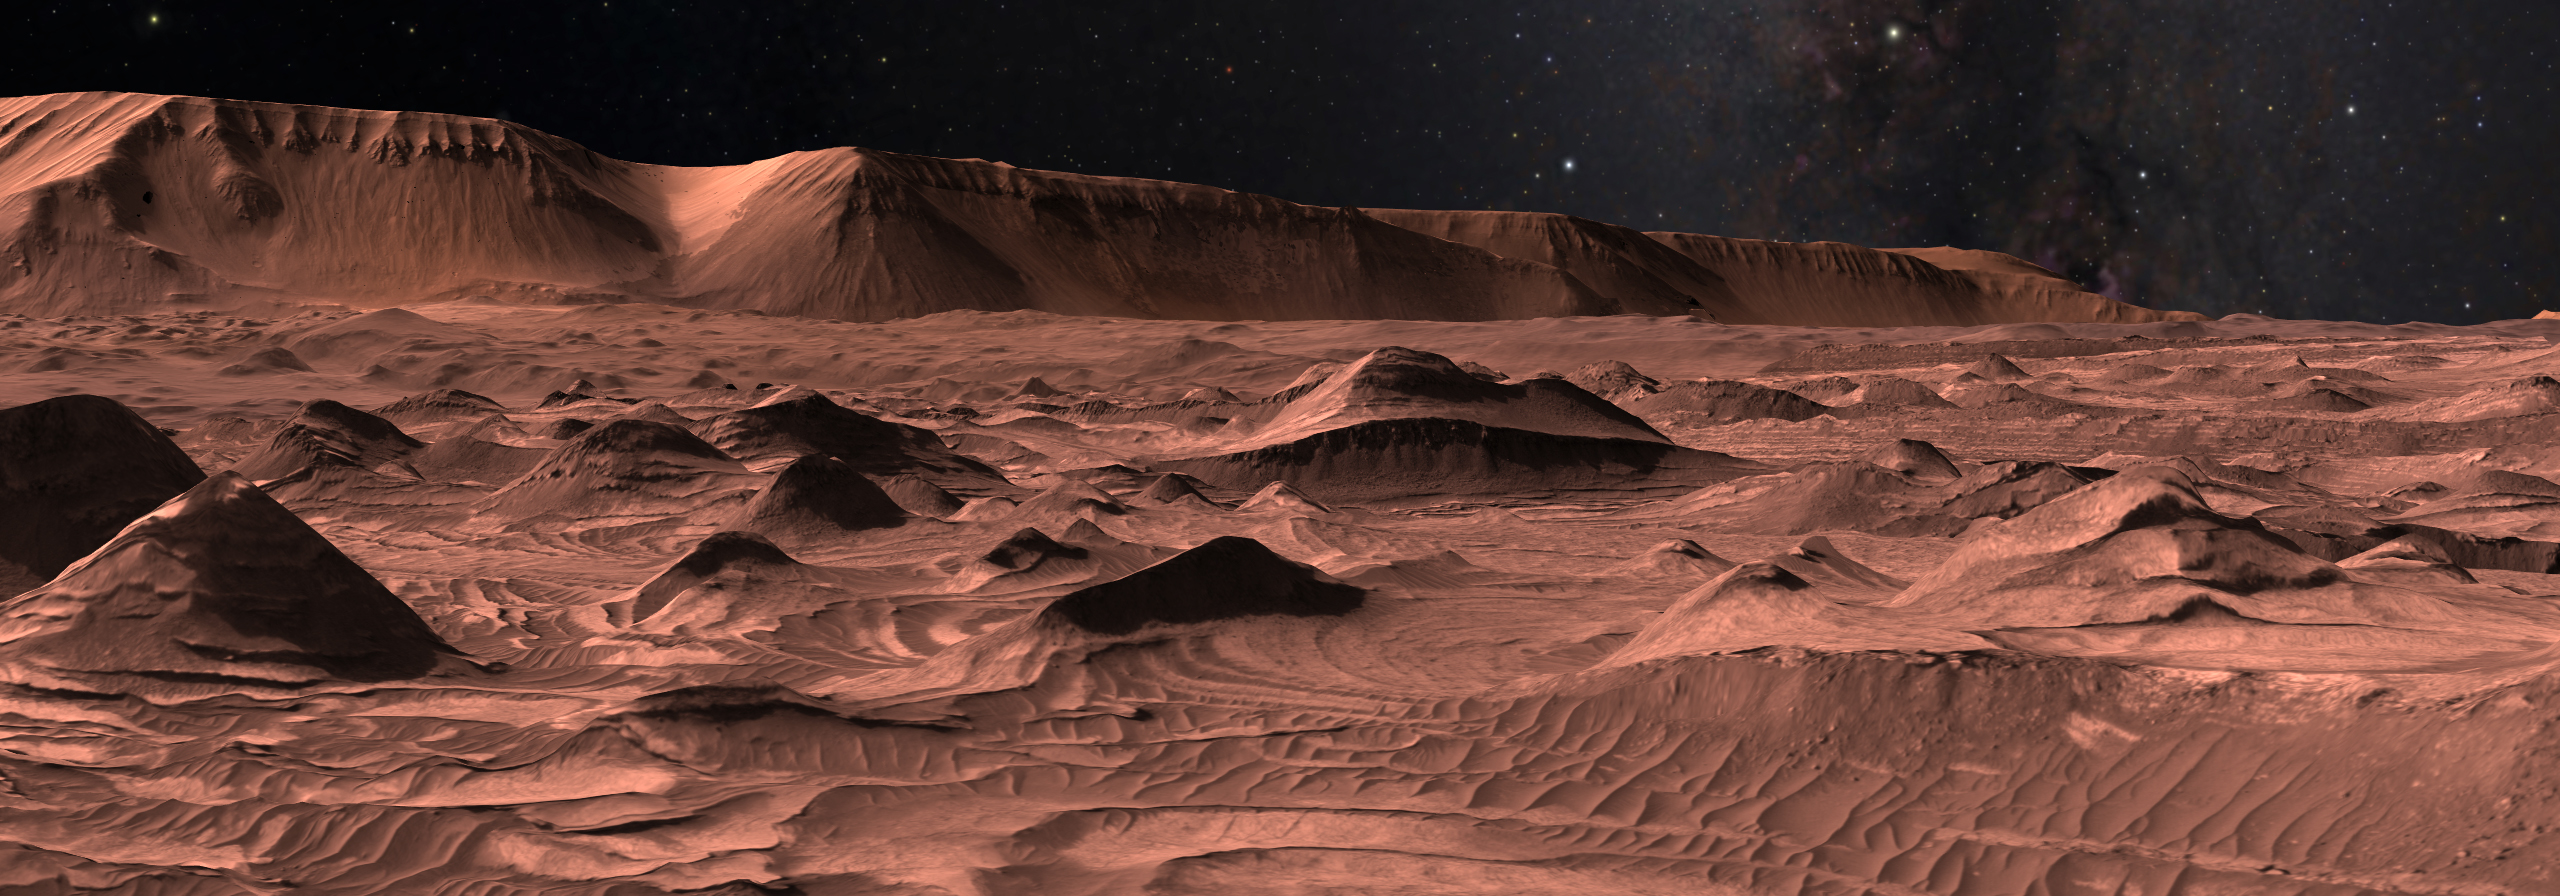
\includegraphics[width=\linewidth, height=0.35\linewidth]{figures/teaser.jpg}
  %\includegraphics[width=\linewidth]{CypressView}
  %\caption{In the Clouds: Vancouver from Cypress Mountain. Note that the teaser may not be wider than the abstract block.}
%	\label{fig:teaser}
}

%% Uncomment below to disable the manuscript note
%\renewcommand{\manuscriptnotetxt}{}

%% Copyright space is enabled by default as required by guidelines.
%% It is disabled by the 'review' option or via the following command:
% \nocopyrightspace

%\vgtcinsertpkg

%%%%%%%%%%%%%%%%%%%%%%%%%%%%%%%%%%%%%%%%%%%%%%%%%%%%%%%%%%%%%%%%
%%%%%%%%%%%%%%%%%%%%%% START OF THE PAPER %%%%%%%%%%%%%%%%%%%%%%
%%%%%%%%%%%%%%%%%%%%%%%%%%%%%%%%%%%%%%%%%%%%%%%%%%%%%%%%%%%%%%%%

\begin{document}

%% The ``\maketitle'' command must be the first command after the
%% ``\begin{document}'' command. It prepares and prints the title block.

%% the only exception to this rule is the \firstsection command
\firstsection{Introduction} \label{sec:introduction}
\maketitle

%\emilcomment{TODO: Need larger labels, cannot read}
%\emilcomment{TODO: Video}
%\alexcomment{TODO: Check Section 4.4}
%\kallecomment{TODO: Add information about Chunk rendering to 4.4}
%\kallecomment{TODO: Add related work about level of detail}
%\alexcomment{TODO: Check 4.5 Cluster Rendering}
%\alexcomment{TODO: Write Results section}
%\kallecomment{TODO: Fix up reference}
%\kallecomment{TODO: Figure 8 caption}
%\alexcomment{TODO: Figure 9 caption}
%\alexcomment{TODO: The submission ID is missing} % Not needed I think, not a double blind review

Throughout history the study of celestial bodies orbiting our Sun has always intrigued mankind and played a central role in mythology, culture, and contributed to the scientific discovery of the fundamental laws of physics.
Since the invention of the telescope in the $17^{\textrm{th}}$ century, our knowledge of the planets and other celestial bodies in our solar system has grown at an ever-increasing rate.
The quest for more knowledge made a leap forward in 1962 when Mariner 2 flew by Venus paving the path for a long-term, and still ongoing, systematic mapping of the solar system by spacecraft flying by or orbiting objects of interest.
Another landmark in the exploration of the solar system was NASA's Viking program, launched in the year 1975, which gathered important information about Mars and its surface features from the two orbiting satellites and the landers put on the surface of the planet.

The flyby of the dwarf planet Pluto by the New Horizons mission in 2015 is yet another milestone as Pluto~\footnote{When New Horizons was launched in 2006, Pluto was still defined as a planet. It has since been reclassified as a dwarf planet.} was the last planet to be visited by a space probe. As a consequence of the spacecraft-based exploration of the solar system we now have detailed surface data from a range of celestial bodies orbiting the sun, including some located in the most remote places of the solar system. 

\begin{figure*}
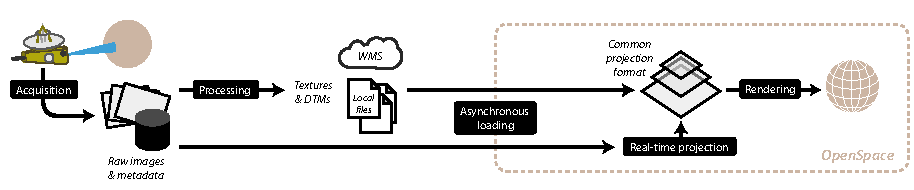
\includegraphics[width=\linewidth]{figures/overview.pdf}
\caption{Illustration of the processing pipeline of the presented application. Raw images acquired from spacecraft can be used as-is, by utilizing orientation information, and projecting images directly onto celestial bodies, or, they can be processed and made available as online global map resources. Our system supports both approaches, as in the cases with Pluto flyby of New Horizons and the several missions to Mars. This puts high demands on the system to interactively render high-resolution images as well as reducing the time from image acquisition to dissemination.}\vspace{-2mm}
\label{fig:procpipe}
\end{figure*}

This large collection of data has enabled numerous scientific discoveries about the geological structure of the planets and many of these have been based on the use of image processing and visualization.
The work presented in this paper focuses on providing visualization tools and applications for communication of these discoveries, and the engineering efforts which enabled them, based on acquired data and interactive visualization.
The developed application is an example of a new data-driven and interactive paradigm of science communication, which provides a means of bridging the gap between experts and the general public, but also serves as a useful tool for communication within a team of experts working on complex missions and scientific exploration.
We are focusing on the use of open surface data made available by the different space agencies and research laboratories from which high-resolution and scientifically accurate representations of celestial bodies are created using geometry extraction and texturing, enabling exploration in \emph{Globe Browsing} sessions.
%Visualization then provides a unique possibility to contextualize scientific exploration of our solar system, as well as the challenging engineering efforts behind space exploration, and, indeed, creates the ability to virtually visit the surface of celestial bodies. 

There are several technical challenges involved in accessing and preparing the data for interactive globe rendering which stem from aspects of collected data such as size, complexity, numerical precision and accuracy, need for curvature corrections, and incompleteness and variety of sources.
Furthermore, the use of multi-resolution visualization approaches to out-of-core data streaming from remote repositories and navigation models spanning from surfaces to interplanetary space requires dynamic data flow and navigation control. 

We have chosen to address the challenges in the context of three representative application scenarios for different celestial bodies.
As a first example we show how our system can enable interactive and seamless surface exploration of Mars with previously unprecedented resolution.
We then show, as an example of temporal data, how the daily images of the Earth, made  available through the NASA GIBS project, can be accessed and visualized from vantage points in interplanetary space as well as in close ups of regions of interest in order communicate dynamic processes on celestial bodies.
Finally, we present how complex data gathering process can be visualized by virtually following the New Horizons fly-by of Pluto in 2015, and tapping into the data flows of the instruments on the probe showing how high resolution image mosaics are constructed, thus dramatically reducing the time between discovery and dissemination.

At the core of our approach lies the gathering of surface image data and projecting it to a common projection format either as a preprocessing step or as an integrated part of the rendering process to visualize the data acquisition.
The datasets are rendered as layers and projected on the surface of globes.
\fig{procpipe} presents an overview of this processing pipeline.
In our work we we adhere to four underpinning principles which guided the design and implementation;

\begin{itemize} 
  \item Visualization should be data-driven, and thus only data derived from the instruments on space probes should be used,
  \item Data from multiple instruments, and/or probes, should be merged to represent the accumulated knowledge of an object,
  \item The maximum available resolution in space and time should be accessible on demand for the areas of interest,
  \item Data should be as current as possible by enabling access to a range of curated and frequently updated repositories.
\end{itemize}

We provide a reference implementation of this system in the open-source astrovisualization framework \emph{OpenSpace}, targeting data exploration and science communication on a range of platforms including large scale dome theaters, virtual reality headsets, and touch tables, and thus enabling spatio-temproal navigation and contextualization of satellites and space probes together with celestial bodies.

Our contributions can be summarized as:
\begin{itemize}
\item A visualization pipeline and platform for contextualized multi-resolution spatio-temporal data of celestial bodies,
\item Tailoring of data handling, visualization, and interaction methods integrated into the pipeline,
\item Three representative application scenarios demonstrating the utility and flexibility of the system.
\end{itemize}


\begin{figure*}
\centering
    \begin{subfigure}{0.33\linewidth}
    	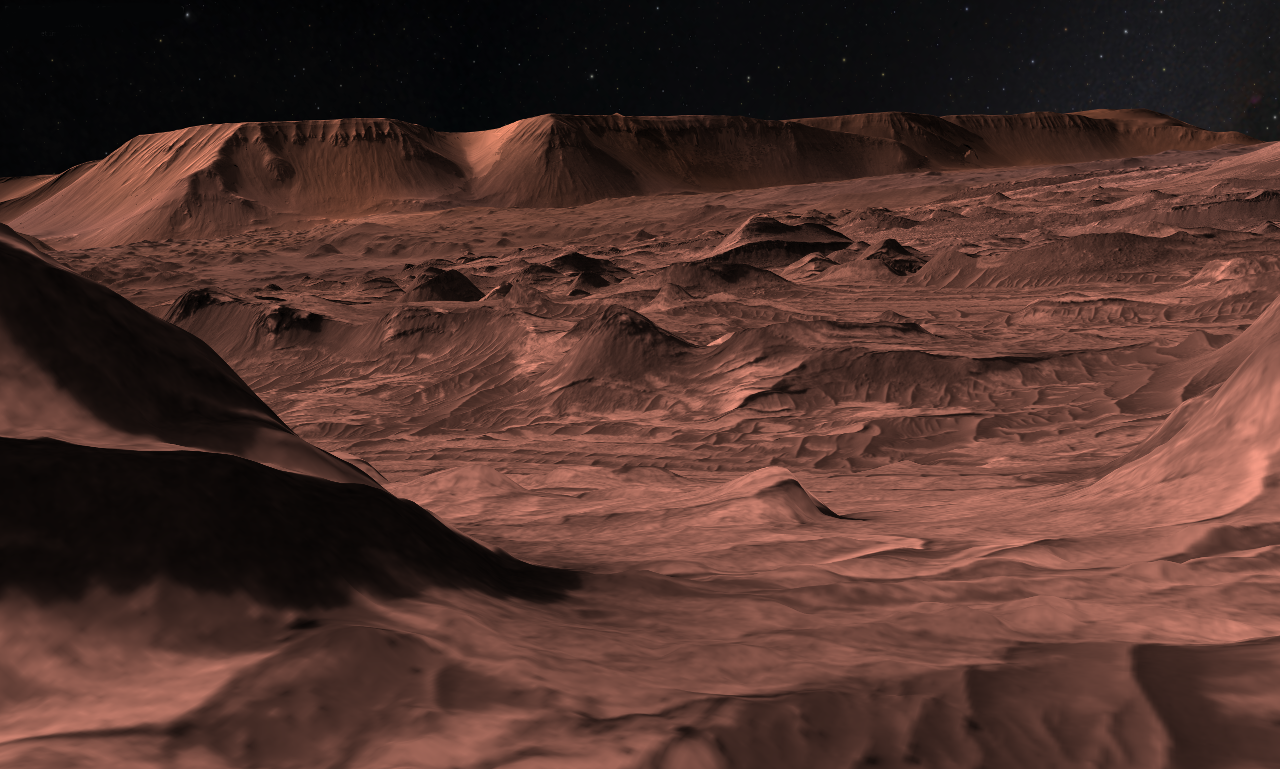
\includegraphics[width=\linewidth, height=0.6\linewidth]{figures/mars.png}
      \caption{Mars}
    \end{subfigure}
    \begin{subfigure}{0.33\linewidth}
    	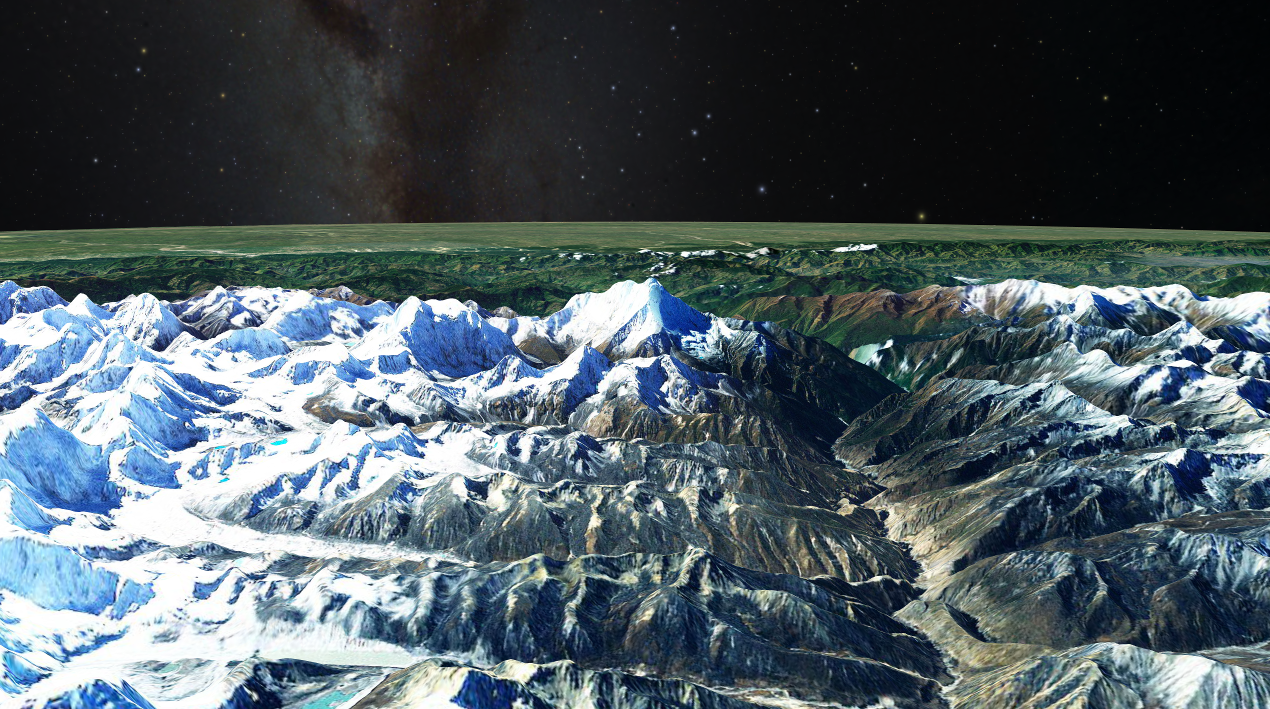
\includegraphics[width=\linewidth, height=0.6\linewidth]{figures/earth.png}
      \caption{Earth}
    \end{subfigure}
    \begin{subfigure}{0.33\linewidth}
    	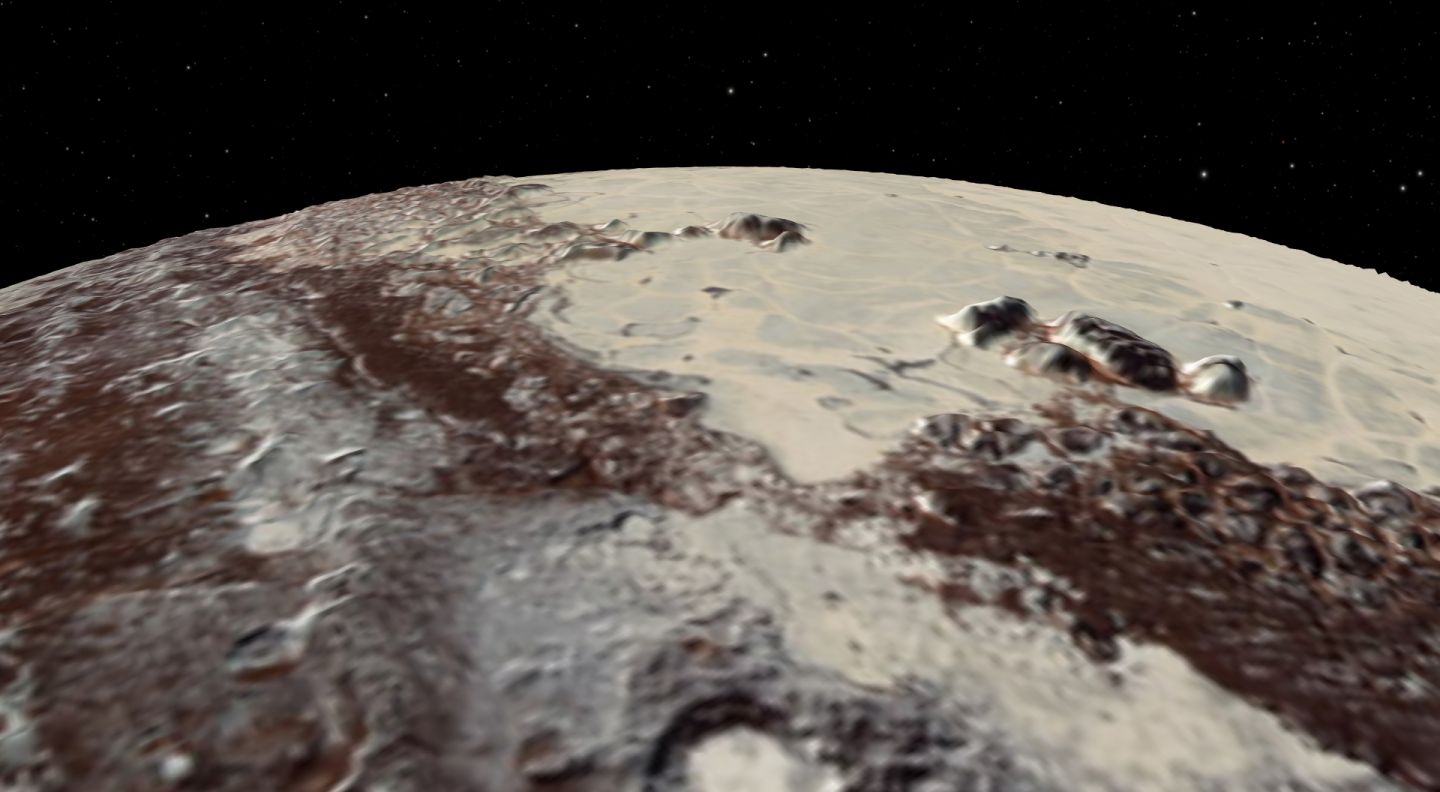
\includegraphics[width=\linewidth, height=0.6\linewidth]{figures/pluto.png}
      \caption{Pluto}
    \end{subfigure}
    \caption{Our system demonstrated with the three described scenarios. High-resolution surface features on Mars (a) showing features with centimeter resolution, dynamic processes on Earth (b), and reconstructed imagery and digital terrain map on Pluto (c). Each of these scenarios are used in public presentations to explain their respective scientific discoveries to public audiences.}\vspace{-3mm}
    \label{fig:scenarios}
\end{figure*}

%%%%%%%%%%%%%%%%%%%%%%%%%%%%%%%%%%%%%%%%%%%%%%%%%%%%%%%%%%%%%%%%
%%%%%%%%%%%%%%%%%%%%%%%%% Related Work %%%%%%%%%%%%%%%%%%%%%%%%%
%%%%%%%%%%%%%%%%%%%%%%%%%%%%%%%%%%%%%%%%%%%%%%%%%%%%%%%%%%%%%%%%

\section{Related Work} \label{sec:relatedwork}

%\begin{enumerate}
%\item Astronomical visualization in general.\plgrem{I will try to compile a general collection of astro vis citations}
%\item Astrovis for communication - planetariums
%2. Go towards Science communication and contextualization.
%\item Related GIS work
%\item LOD - look up the real references from the LOD book. It is not OK to refer to pages in the book.
%
%\end{enumerate}

The presented application builds on technologies and methods that we have arranged into four major topics, namely large-scale astronomical visualization, science communication, geographical information systems (GIS), and level-of-detail (LOD) rendering methods for (planetary scale) terrains. Our review of related work thus follows the same structure where we outline previous methods and approaches and conclude with commentaries on how it relates to the presented application.

%Our application builds on previous work in the fields of large-scale astronomical visualization, geographical information systems (GIS), and level-of-detail (LOD) rendering.

\noindent\textbf{Astronomical Visualization} --
One of the challenges in astrovizualization is to deal with positioning and navigation over extreme distances and there are several papers describing appproaches to this this problem such as the the notion of a ScaleGraph introduced by Klashed \etal~\cite{KHECY10}, who describe an implementation from 2003. The concept of \emph{power scaled coordinates} (PSC), introduced by Hanson~\etal, addresses large scale differences in astrovisualization and animations~\cite{hanson2000very} and subsequently Fu~\etal~\cite{fu2006navigation} categorized the problem of large scale navigation and positioning. Fu and Hanson also introduced a depth buffer remapping to cover a wider range of distances than possible with a fixed point depth buffer and conventional near and far planes~\cite{fu2007transparently}. Other efforts include the work by Li~\etal~\cite{li2006scalable} who introduce a world-in-miniature techniques based on logarithmic landmarks for navigation support using PSC. In our presented work, we use the Dynamic Scene Graph as proposed by Axelsson \etal~\cite{Axelsson2017Dynamic}, as it allows for seamless navigation across large distances without loss of precision.
There are several other contributions to the visualization field with astrophysics as its motivation such as the work on visualization on relativity by Weiskopf~\etal~\cite{weiskopf2005visualization} and the multiwavelength data visualization by Li~\etal~\cite{li2008visualizing}. An examples of how visualization has played a documented role in the scientific exploration is the work on interactive visualization of galaxy surveys by Punzo~\etal~\cite{punzo2015role}.

%%% End of paste from Alex, start of Alex's previous notes.
Relevant to the presented work here is a number of freely available astronomical software packages such as Eyes on the Solar System by NASA~\cite{hussey2010eyes}, also tools for planetary rendering in free software such as Blender~\cite{kent2013visualizing, naiman2016astroblend} can provide engaging experiences for a wide range of users.

\noindent\textbf{Science communication} --
Visual communication and the use of animations and interactive techniques are immensely valuable and enable a wide appeal across ages and cultures.
Computer graphics and interactive visualization techniques are at the core for communicating scientific findings and contextualizing information.
Notable examples of applications in which huge scale-differences are visualized include movie productions, a classic example is \emph{Powers of Ten} by Eames~\cite{powersOfTen} from 1977, but include current interactive software packages such as Uniview~\cite{KHECY10}, DigiStar~\cite{ES16}, and DigitalSky~\cite{Sky16}, which are all based on curated datasets containing information about our universe~\cite{abbott2006digital}. 
Another more recent effort by Weiskopf~\etal~\cite{weiskopf2006explanatory} aims at an explanation of the special and general relativity.

Virtual reality environments such as planetariums~\cite{magnor2010progress, liu20013} have always been in the focus of educators, but a shift towards supporting data inspection on consumer grade hardware is ongoing~\cite{nakasone2009astrosim}.
Recent advances in graphics hardware and processing power in consumer hardware has enabled a broad use of actual scientific data in applications aimed for science communication for the public at science centers and elsewhere.
One such story is presented by Ynnerman~\etal~\cite{ynnerman2016interactive}.
The ability of providing the same data as scientists have used in their explorations to the layman user is currently a major change and a paradigm shift in science communication.


%Geospatial Data Abstraction Library (GDAL) is an open source software package and C++ library enabling re-projection and warping of map datasets and can act as a layer of abstraction between the rendering software and the many different types of map formats and projections.

\textbf{Geographic information systems (GIS) -- } GIS relies heavily on the ability to gather, transform, and visualize data with geospatial information.
Texture maps and digital elevation models (DEM's) are typical examples of such data and research and development of software solutions to handle different parts of GIS, such as rendering, have lead to different applications in space visualization.

A GIS software should be able to handle a vast amount of projection formats. When it comes to globe rendering, however, there are standards that are more common than others.
Equirectangular geographic projection is by far the most commonly supported format used for unprojection of globes, and also plays a major role in applications outside of computer graphics, such as the Global Positioning System (GPS) \cite{cozzi20113d}.

Geographic projection suffers from a couple of well known issues near the poles such as oversampling and polar pinching \cite{cozzi20113d}. The number of available data products for this format, however, makes it useful for our purposes.

\noindent\textbf{Level-of-detail (LOD)} --
LOD and multiresolution methods are crucial when visualizing and navigating across large datasets~\cite{luebke2003level}.
By using representations with fewer vertices and lower resolution textures to render distant objects, more resources can be directed towards rendering salient objects.
Cozzi and Ring \cite{cozzi20113d} provide a comprehensive introduction to the most common methods used for globe rendering.
Examples of earlier LOD techniques for globe rendering include the real-time optimally adapting meshes (ROAM), introduced by Duchaineau~\etal~\cite{duchaineau1997roaming}, with improvements made by Hwa~\etal~\cite{hwa2005real}, similar to P-BDAM by Cignono \etal~\cite{cignoni2003planet,cignoni2003bdam}. With todays hardware these methods does not allow full GPU acceleration and are thus prompted for more GPU-friendly techniques, such as chunked LOD \cite{ulrich2002rendering} and geometry clip-maps \cite{losasso2004geometry}.

Erikson \etal~\cite{Erikson:2001:HFD:364338.364376} describe a hierarchical LOD (HLOD) method generalized for three-dimensional geometries. For two-dimensional geometries, such as chunks on a globe where each leaf node in a quad-tree, describing the complete object, corresponds to a part of the complete globe at a specific detail level.
The quad-tree is dynamic and able to update its nodes by procedures known as splitting and merging so that high LOD is used only where it is needed.

Ulrich~\cite{ulrich2002rendering} proposed a chunked LOD technique where geometry generation of each chunk requires preprocessing.
In Ulrich's implementation, the generation process is separated from the run-time selection of detail levels. Cozzi and Ring \cite{cozzi20113d} define sub-processes of chunked LOD rendering as \emph{selection} and \emph{switching} which we adhere to.

%Early contributions by R{\"o}ttger \etal~\cite{rottger1998real} showed height field rendering using LOD methods.

We adopted the chunked LOD method due to its GPU friendly nature and implicit handling of polar issues that is common for geometry clip-maps. In contrast to Ulrich \cite{ulrich2002rendering}, we generate geometry dynamically on the GPU using vertex texture sampling. This is to enable dynamic loading of different terrains. These can be \emph{digital elevation models}~(DEM's) or \emph{digital terrain models}~(DTM's) \cite{li2004digital} generated from data gathered from altimeters or stereo images.


%To enable dynamic loading of height maps we use a light weight implementation of the chunked LOD method where geometries are generated on the fly. See Section \ref{sec:chunktree}.


Important optimization techniques for culling of HLOD are clearly described by Cozzi \cite{cozzi2008visibility}. Horizon culling and view frustum culling are important procedures for our purposes since the techniques vastly reduces the number of chunks that need to be rendered without compromising the image quality.

%%%% MISSING CITATIONS on Terrain Rendering (planetary scale)
%Planet-sized batched dynamic adaptive meshes (P-BDAM\cite{cignoni2003planet}. -- missing
%Survey of semi-regular multiresolution models for interactive terrain rendering \cite{pajarola2007survey}. -- missing
%GPU-friendly high-quality terrain rendering\cite{schneider2006gpu}. 
%Seamless patches for GPU-based terrain rendering \cite{livny2009seamless}. -- missing!
%Planetary-scale terrain composition\cite{kooima2009planetary}. -- missing!

%%%% INCLUDED CITATIONS on Terrain Rendering (planetary scale)
%BDAM—Batched Dynamic Adaptive Meshes for high performance terrain visualization  \cite{cignoni2003bdam}. -- OK!
% Geometry clipmaps: terrain rendering using nested regular grids\cite{losasso2004geometry}. -- OK!
%Real-time optimal adaptation for planetary geometry and texture: 4-8 tile hierarchies\cite{hwa2005real}. -- OK!
%Real-time generation of continuous levels of detail for height fields\cite{rottger1998real}. -- OK!

%Height map datasets can be generated using measured data from altimeters on the satellites, corrected to match an offset from a reference ellipsoid in the direction of the geodetic normal for every point on the surface covered by the dataset.
%Height maps can also be generated using stereoscopic reconstruction.

\noindent\textbf{Stereoscopic Reconstruction} -- Although it is only tangentially related to the system that we are proposing, it is valuable to place the many ongoing efforts in the reconstruction of geometry from multiple image sources into context. Koch \cite{Koch95} provided a framework to analysis a scene using a dense depth maps and constructing triangulated surfaces from surface points. This work spawned a large number of interesting research that is outside the scope of this manuscript. Wolf \etal~\cite{wolf2000elements} provide a useful overview over the field of using photogrammetry and stereoscopic reconstruction for terrains.


%\begin{enumerate}
%\item the book 3D Engine Design for Virtual Globes
%\item terrain renderer
%\item 3d reconstruction from images (stereoscopic and structure-from-motion)
%\item GDAL
%\item ``virtual presence'' systems
%\item What else?
%\end{enumerate}
%Length: About 1 page\\
%Note:  The page limit was increased to 9+2 pages this year (= 9 pages of manuscript, 2 pages of references). So we should make use of this and cite the hell out of everything that's related


%%%%%%%%%%%%%%%%%%%%%%%%%%%%%%%%%%%%%%%%%%%%%%%%%%%%%%%%%%%%%%%%
%%%%%%%%%%%%%%%%%%%% Application Scenarios %%%%%%%%%%%%%%%%%%%%%
%%%%%%%%%%%%%%%%%%%%%%%%%%%%%%%%%%%%%%%%%%%%%%%%%%%%%%%%%%%%%%%%

\section{Data Scenarios and Acquisition} \label{sec:scenarios}
The available surface data is the underpinning resource upon which our framework is relying. In this section we therefore provide an in-depth presentation of the data behind the three application scenarios we present in this paper.
We begin by describing the acquisition of terrain data with a high spatial resolution but limited temporal resolution for Mars (Section~\ref{sec:scenario:mars}). We then given an overview of the dynamic time-varying data for Earth (Section~\ref{sec:scenario:earth}). The section is concluded with a description of on-line image acquisition of a non-orbiting spacecraft, exemplified by New Horizons flyby (Section~\ref{sec:scenario:pluto}) of Pluto.
\fig{scenarios} shows examples of these three application scenarios.

%We chose three distinct application scenarios that cover the majority of planetary surface visualization use cases in the solar system.
%In this section we describe the terrain data we visualize with a high spatial resolution but limited temporal resolution on Mars (Section~\ref{sec:scenario:mars}), the visualization of temporal phenomena on Earth (Section~\ref{sec:scenario:earth}), as well as the on-line image acquisition of a non-orbiting spacecraft, exemplified by New Horizons (Section~\ref{sec:scenario:pluto}) at Pluto.

%For each of the scenarios, we provide information about the data sources and how these provide specific challenges for a terrain rendering system.

\subsection{Mars} \label{sec:scenario:mars}
%From the pictures of the first Mars missions (Mars 2, Mars 3, Mariner 9), no other planet in the solar system has gained as much attention from the different space agencies.
So far 14 orbiters and 13 landers that have been sent to our neighboring planet Mars, which is now the most intensively investigated planet beyond the Earth-Moon system and a vast dataset of planetary imagery has been acquired.
The most important large scale imaging campaign of Mars is carried out by the Mars Reconnaissance Orbiter (MRO), equipped with an array of cameras, spectrometers, and radar used to image the surface at different resolutions in part for scientific discovery, as well as for the use in landing site evaluation ~\cite{zurek2007overview}.
The spacecraft is in a polar orbit which means that, as the planet rotates underneath it, the instruments will eventually be able to perform measurements at every location on the planet.

The \emph{Mars global digital image mosaic}~(MDIM) is a global image dataset with a resolution of up to 240\,meters/pixel~\cite{archinal2003mars}.
The latest version of this image mosaic, MDIM 2.1 is compiled from a set of Mariner 9 and Viking images with improved accuracy as a result of constraints from the \emph{Mars Orbiter Laser Altimeter} (MOLA) data from the Mars Global Surveyor (MGS) spacecraft.
The DEM, assembled from MOLA data, provides an offset from the \emph{Areoid}, Mars' reference ellipsoid, to an average vertical precision of ~100\,meters with a resolution of about 450\, meters/pixel~\cite{smith2001mars}.
This global height map provides sufficient resolution to serve as a background for other reconstructed local terrain models.

The \emph{Context Camera}~(CTX) on the MRO provides gray-scale images of the planetary surface with about 6\,meters/pixel resolution used for providing contextual information for the other instruments observing the Martian surface~\cite{zurek2007overview}.
NASA Ames Research Center assembled a 5\,TB global mosaic of CTX data with roughly 70\% surface coverage.
Currently the CTX camera has mapped over 99\% of the Martian surface after the MRO has finished 50000 orbits.

The \emph{HiRISE} camera on the MRO provides images with a spatial resolution of 25\,cm/pixel that have been used to select and evaluate potential landing sites~\cite{mcewen2007mars}.
Both the CTX and HiRISE images can be used for stereoscopic reconstruction of DTM's that are available as local areas of interest on the surface (see Section~\ref{sec:processing}).
McEwen \etal~\cite{mcewen2016people} describes the HiRISE data available online and how the public can contribute in the choice of future target locations.

The main challenges in the Mars browsing application scenario stem from the need of handling multiple data products at various resolutions in a single context.
This requires layer handling and the ability to dynamically read map data and seamlessly render it with varying levels of detail.
% The accuracy constraints calls for an ellipsoidal globe model where high precision rendering is needed to enable the rendering of high resolution local map and terrain data together with global datasets.

\subsection{Earth} \label{sec:scenario:earth}
A vast number of data sources of varying spatial and temporal resolutions are available for Earth.
Even though the thick atmosphere makes the acquisition of detailed surface features difficult, the relative ease of placing a satellite into orbit has resulted in currently hundreds of active Earth observing satellites.
Furthermore, a major design constraint for interplanetary spacecraft is the available bandwidth through the \emph{Deep Space Network}, limiting the amount of data that can be recovered.
This design constraint does not apply for Earth orbiting satellites and it thus enables the creation of high spatial and temporal resolution imaging; in most cases these are global images which are updated daily, but more local and higher resolution satellites exist, such as the geostationary GOES-16 which captures an image of the entire western hemisphere every 15 minutes at 10000$\times$10000 pixels.

We have focused on three sun-synchronous satellites, described below, returning daily images of Earth, each covering the majority of Earth's surface area.
The satellites perform scans in a large wavelength spectrum, covering both visible light as well as infrared light ($\approx$~400\,nm~--~14\,\textmu m) and thus provide ample ground for public communication of studies of the surface, oceans, biosphere, and atmosphere.
These datasets are available through a public interface provided by the NASA \emph{Global Imagery Browse Services}~(GIBS) that provides a unified interface to make NASA and NOAA imagery available to the general public via \emph{web map services}~  (WMS)~\cite{cechini2013expanding}.

The \emph{Moderate Resolution Imaging Spectroradiometer}~(MODIS) instrument is used on the \emph{Terra} and \emph{Aqua} satellites since 1999 and 2000.
Its resolution varies between 250\,meters/pixel and 1\,km/pixel~\cite{salomonson1989modis, justice2002overview} and a global image has been generated each day since 2000.
The data is used for showing land boundaries, cloud movements, the study of phytoplankton, and global temperature studies, providing a unique view into the dynamic nature of our planet over this large timespan.
% Due to a limited field of view, the instruments do not have full coverage of the planet at the equator, leading to striped areas of missing data (see Figure?).

The \emph{Visible Infrared Imaging Radiometer Suite}~(VIIRS) instrument on the Suomi NPP satellite provides comparable data to the MODIS instrument and has provided spatial resolutions between 375 and 750 \,meter/pixel since 2012~\cite{schueler2002npoess}.
In addition, it has a pan-chromatic Day-Night-Band which is used to measure the night side of the Earth, thus creating the ability to study the development of cities on Earth.
% compared to the MODIS instrument has a wider field of view, allowing a continuous coverage of the Earth at all latitudes without missing data.

The main challenge in handling time varying map data is the ability to cache a buffer of data read asynchronously.

\subsection{Pluto} \label{sec:scenario:pluto}
The images of the previous two scenarios were acquired by orbiting satellites providing the ability to produce images for an extended periods of time.
% In the previous two scenarios the global images were acquired by orbiting satellites that produce images for an extended period of time.
As these orbits are designed to have a low eccentricity, the instruments' surface resolution is constant throughout the orbit, which is very useful when reprojecting images to be used in global maps.
However, not all spacecraft-based image acquisitions are performed from close to circular orbits.
One recent example of a non-orbiting mapping campaign was performed in July 2015 by the New Horizons spacecraft as it was flying past the dwarf planet Pluto.
Prior to the flyby, the best images of Pluto were available from Hubble with a resolution of about 161\,km/pixel.
The main image acquisition instrument on board New Horizons is the \emph{Long Range Reconnaissance Imager}~(LORRI), a gray-scale telescope.
The \emph{Ralph} instrument's primary data source is a Multispectral Visibile Imaging Camera~(MVIC) enables the recovery of spectral information and thus provides color information for the LORRI images.
The \emph{Radio Science Experiment}~(REX) is part of the radio communications system and has the ability to detect radio emissions either directly from Pluto's surface, thus measuring its surface temperature, or Earth-based radio signals that pass through Pluto's atmosphere and thus measure its composition.
Between January and July, the surface resolution of the LORRI instrument gradually increased, reaching about 1\,km/pixel on the day of the flyby and peaking at 50\,meters/pixel during the time of closest approach.

The time varying resolutions provide an opportunity to show the incremental image acquisition to the general public, rather than using a static planetary map of varying resolution. Navigation data and image metadata made available by the New Horizons team makes it possible to show the spacecraft's data acquisition process in the context of Pluto and its moons.

%We chose New Horizons as the third scenario due to this challenging varying resolution between image campaigns which is not normally present in other surface mapping projects.
%Furthermore, the varying resolutions provide a opportunity to show the incremental image acquisition to the general public, rather than using a static planetary map of varying resolution.

%%%%%%%%%%%%%%%%%%%%%%%%%%%%%%%%%%%%%%%%%%%%%%%%%%%%%%%%%%%%%%%%
%%%%%%%%%%%%%%%%%%%%%%% System Overview %%%%%%%%%%%%%%%%%%%%%%%%
%%%%%%%%%%%%%%%%%%%%%%%%%%%%%%%%%%%%%%%%%%%%%%%%%%%%%%%%%%%%%%%%

\section{Globe Browsing System} \label{sec:overview}
In this section, we describe aspects of the overall processing pipeline (see \fig{procpipe}) and the technical details required for the three representative application scenarios described in the previous section.
As there are two distinct pathways into the rendering component, some of the scenarios utilize only parts of the described pipeline. More specifically, real-time projection does not utalize tiled textures.

The following sections elaborate on the individual components of our system that are required to provide access to a large variety of imagery sources.
First, the \emph{Data Access}~(Section~\ref{sec:dataaccess}) discusses the different ways through which the data is accessed in our system.
Second, the \emph{Data Preparation}~(Section~\ref{sec:processing}) of acquired data is described that might be required if the images are not available in the correct georeferenced projection format or when detailed digital terrain models have to be generated.
Third, if the scenario requires an iterative image projection and navigational data is available for specific mapping campaigns, a \emph{Real-time projection} is performed in the system.
Section~\ref{sec:imageprojection} describes the unprojection of these images.
Last, a \emph{level-of-detail surface rendering} is performed utilizing the common projection format.
Section~\ref{sec:renderingsystem} elaborates on the details of this rendering pipeline.

In order to be able to read as many data sources as possible without the need for additional reprojection steps, we chose to use a standardized common georeferenced map projection format; namely the equirectangular geographic projection~\cite{snyder1997flattening}.
From this georeferened coordinate system, the renderer transforms vertices to achieve the correct mapping of the globe.
This makes use of an inverse projection $(x,y,z)^T = P^{-1}(\phi, \theta)$ that maps each geodetic coordinate defined by a latitude ($\phi$), and a longitude ($\theta$) to a Cartesian coordinate on the surface of the reference ellipsoid in the model space of the celestial body.
For Earth, this is a transformation from the geographic projection on the Geoid to the commonly used World Geodetic System 1984 (WGS84) coordinate system~\cite{decker1986world}.
%For Mars, inversely project the reference Arenoid~\cite{seidelmann2002report}, whereas Pluto's reference ellipsoid has been adapted based on the images acquired by New Horizons~\cite{stern2015pluto}.

\subsection{Data Access} \label{sec:dataaccess}
All of the data that can be accessed using our system has to be presented as image data.
While this might place a constraint on the data types that can be visualized, it is in most cases possible to represent the interesting information as gray-scale images instead, for example digital terrain models, where the pixel information corresponds to a height offset from a reference ellipsoid.

The most common access pattern for global image sources is a web-based LOD service called the \emph{Web Map Service}~\cite{open2006opengis, maso2010opengis}.
While there are different dialects of this standard, it is possible to query a web server for an image covering a specific portion of a celestial body.
One common dialect is the \emph{Tile Map Service}~(TMS) which provides access into an image quad-tree containing the global imagery at different resolutions.
Each tile for the desired resolution level can then be requested individually.
The access to these online datasets in our system is unified through the use of the \emph{Geospatial Data Abstraction Library}~(GDAL)~\cite{warmerdam2008geospatial}, which enables the access to a variety of WMS dialects through a single interface, thus drastically increasing the number of datasets that are accessible.

When reading regional datasets delineated by a longitude-latitude bounding box, GDAL also provides a unified interface through the use of \emph{virtual datasets} which enables remapping of data and reinterpretation of data types.
The interface supports a vast amount of data types including common ones such as IMG, GeoTiff, and Cube files.
This support enables the system to load these datasets without the need for an Internet connection, which might not be available or fast enough at some locations.

In the case of iterative image projections, such as in the New Horizons scenario, the individual images can be loaded as they are produced and released by the science team.
Since these images are usually not georeferenced, real-time information about the spacecraft and its instruments are used in order to project these images, as described in Section~\ref{sec:imageprojection}.

\subsection{Data Preparation} \label{sec:processing}
Before the image datasets can be rendered some of the data need to be prepared.
This section describes these preparation steps for these datasets which might occur as a separate preprocessing step or during the rendering, depending on the source and extent of the data.

% either as a preprocessing step or during the rendering, depending on the source and extent of the data.
% While some data sources might require preparation, other might be usable without 

\noindent \textbf{Projection Formats. } For the case of global image datasets, a variety of geographic projection formats are available.
In order to support the layering of multiple data sources for a multimodal surface visualization, we chose to employ the most widely used format, the equirectangular geographic projection, as a single unified projection format for the planets in our system.
If a global image dataset is not provided as an equirectanglar projection, we convert the dataset using GDAL.
%Depending on the availability of the data or potential size constraints, the system can be configured to either perform these conversions as a preprocessing step, thus improving the access speed at the cost of increased storage requirements, or at run-time, thus removing the need for a preprocessing step. \kallecomment{This is false!!}

\noindent \textbf{Digital terrain models. } Some spacecraft contain altimeters that are capable of measuring the height information of the planet directly.
In these cases, the height information is presented as a gray-scale image that can be accessed using the methods described previously (see Section~\ref{sec:dataaccess}).
However, most spacecraft do not possess instrumentation that produces direct measurements of height information, for example the CTX and HiRISE on the Mars Reconnaissance Orbiter or the LORRI camera on New Horizons.
In these cases, a digital terrain model can still be reconstructed by using stereoscopic pairs of images in stereophotogrammetry.
The use of the NASA Ames Stereo Pipeline (ASP) stereogrammetry software~\cite{moratto2010ames} for content creation becomes a valuable tool in our pipeline for building DEM's from stereo pairs.
ASP works in tandem with planetary mapping methods available through the United States Geological Survey's~(USGS), \emph{Integrated Software for Imagers and Spectrometers}~\cite{gaddis1997overview}.
CTX patches have successfully been generated from stereo pairs to match the MOLA base map of Mars~\cite{broxton2008ames, mayer2016integrated}. We exemplify this using a collection of CTX images covering West Candor Chasma in Valles Marineris on Mars.
Furthermore, it has been shown to work on reconstructing high resolution DTM's using pairs of the HiRISE camera resulting in a resolution of about 1\,m/pixel~\cite{li2011rigorous}

\subsection{Real-Time Image Projection} \label{sec:imageprojection}
In order to support the direct iterative visualization of spacecraft image acquisition, our system interfaces with various tools used in space mission planning and monitoring.
This information is used to reconstruct the location and orientation of a spacecraft, together with specifications about the instruments camera system, such as field-of-view or detector sizes.
Utilizing this information, together with the timing at which a specific image was taken, we project this image and store it in an equirectangular global image map of the entire globe. This map can then be used as a data source providing image data to the renderer.

The SPICE toolkit provided by NASA's Navigation and Ancillary Information Facility (NAIF) is used to load location and orientation data for planets, spacecraft and instruments~\cite{acton1996ancillary}.
%From this data, we acquire accurate positions and orientations of celestial bodies as well as spacecraft and their instruments throughout the time of a space mission.
Information about image acquisition and exposure time are either directly provided by the mission scientists or are available through NASA's Planetary Data System, which curates information about all past and current space missions~\cite{mcmahon1996overview}.

In order to map image data onto a latitude-longitude format used for rendering, we combine position and navigation data from SPICE with image exposure timestamps from PDS. For individual instruments on the spacecraft, virtual camera frustums are constructed. For each image taken by an instrument, latitude-longitude values of the planetary surface are mapped to image coordinates.
The images are projected to the celestial body using projective texturing as described by Everitt~\etal~\cite{Everitt:2001tg}.
Using this method the planet's triaxial ellipsoid is rendered from the view point of the instrument and then applying the image to the projected planet, thus the image will be applied with the correct geometric distortions and the results is converted into an equirectangular global map.

\subsection{Rendering System} \label{sec:renderingsystem}

The rendering system is primarily driven by rendering of chunks, which are organized into a quad-tree and each chunk covers a particular geographic area of the planetary surface. The processing pipeline is outlined in \fig{chunkproc}. First the tree is processed to reflect the best fit for the given camera view, in this process the chunk tree is evaluated and chunks are either culled or split into child nodes. The resulting leaves are flagged for rendering, as detailed below in Section~\ref{sec:chunktree}. Second, the system requests tile data from tile providers and will continue to render chunks with the currently available tiles, which we explain in Section~\ref{sec:tilemgmt}. Finally, tiles and layers are combined in the fragment pipeline, presented in Section~\ref{sec:chunkrendering}.
Each chunk is rendered individually as a skirted regular grid mesh associated with a geodetic area and level of detail, see \fig{chunks-and-tiles}. The grid size is constant per chunk and the height map layers will affect the altitude of the grid vertices.


Separating the quad-trees that are used for the chunks (the geometry) from the individual tiles (the textures) enables a dynamic loading of information as the geometry LOD can be updated independently from the image information and does not rely on the availability of image information.
This is particularly important when multiple layers are combined that each may have independent resolutions, such as surface image information and height information.
\fig{chunks-and-tiles} shows this exemplified on a single chunk that is rendered using three layers, each organized in a separate quad-tree.

%Each layer originates from a separate dataset and can be enabled or disabled to show how individual instruments have contributed to our knowledge about a celestial body.
% Each layer is assigned to a specific layer group that defines how the layers are blended in the fragment pipeline.
% Examples of layer groups are: height layers, color layers, color overlays, gray-scale layers, gray-scale overlays, night layers and water masks.
% 
%The chunked LOD globe takes care of updating the chunk tree and evaluating the levels of its nodes.
%It also performs chunk culling as well as rendering of individual chunks.
% 
% In our system, a chunk $C\{x, y\}_k$ is a .
% 
%associated with a set of tiles $T_L\{x, y\}_k$ from all active layers L. \emilcomment{examples instead?}
% 
% 
%\plgrem{The Chunked LOD quad-tree needs a better introduction, but should be outlined in related work. It seems Chunk tree is intended to be detailed in 6.2, so either we simply provide an outline here and do a fwd ref to section Chunk Tree. Rewrite this intro when subsections are written.}
%\kallecomment{Moved introduction of chunked LOD tree to related work. Do you think that description is enough?}
% 
% Using a chunked LOD quad-tree structure, each chunk, unprojected on the reference ellipsoid, can be rendered individually.
% The chunk renderer uses a skirted grid \cite{ulrich2002rendering} which can be mapped on to a geodetic region and rendered in place using one or several layers for texturing or height mapping.
% A geographic tessellation defines the unprojection mapping of the chunks.
% 
% A given tile of index $T_L\{x,y\}_{level}$ does not belong to a specific chunk of index $C_L\{x,y\}_{level}$. Instead, one chunk can be rendered using many tiles, even from the same layer as illustrated in Figure \ref{fig:chunks-and-tiles}. This is useful when performing level blending. See section \ref{sec:fragment_blending}. Examples of tile indices used for different layer types is illustrated in Figure \ref{fig:chunks-and-tiles}.

\subsubsection{Chunk Processing} \label{sec:chunktree}
%The quad-tree containing the chunk information is lightweight as 
\begin{figure}
  \centering
    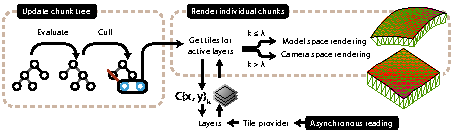
\includegraphics[width=0.5\textwidth]{figures/rendering-pipeline.pdf}
  \caption{Chunk tree processing and rendering pipeline overview. For each frame the tree is evaluated and culled before rendering. Tiles are loaded asynchronously to avoid stalling the rendering pipeline.}  \vspace{-4mm}
%  \caption{Chunk tree processing and rendering pipeline overview.}
  \label{fig:chunkproc}
\end{figure}


% The \emph{Chunk Tree} contains level-of-detail structure of chunk information. 
%The quad-tree storing the chunk information 
%Since we generally do not perform any preprocessing to generate geometries, height mapping is performed on the fly.

Chunk nodes are organized as a quad-tree and defined as $C\{x, y\}_k$ for a surface coordinate $\left( x,y \right)$ and detail level $k$.
Chunk tree evaluation involves selection of desired LOD, limiting the level, and culling of chunk levels, as illustrated in \fig{chunkproc}.
The remaining chunk tree nodes are flagged as visible for rendering.

%Our chunk tree structure is light weight as it does not require vertex data to be stored for every chunk node. We adhere to the common techniques used for chunked LOD rendering but tailor it to our light weight implementation.


\textbf{Chunk selection} is performed by choosing an error metric defined for each chunk, uniquely calculated by the logarithm of the inverse distance from its closest point to the camera position or by an approximation of the projected area of the chunk on a sphere around the camera.
The spherical projection becomes important when using multi-display systems where there should be no difference in the error metric of a specific chunk rendered across two neighboring screens.
These approaches do not need the geometry to be generated in order to calculate a static error metric.

\textbf{Level limitation} is used in case a specific tile dataset does not contain any higher resolution tiles.
Since the geographical extents of the map datasets are unknown until a tile reading procedure is performed there is no way to know the highest detail level beforehand.
To avoid unnecessary splits of chunk nodes, they should not split unless there is higher resolution data available, that is, if a tile reading operation fails.

\textbf{Chunk culling} is performed to minimize the number of render calls due to invisible chunks.
For horizon culling we use the maximum height of the chunk as bounding sphere.
Chunks that are outside of the camera frustum are culled by testing a viewspace defined axis aligned bounding box of the chunk against the camera frustum.
To perform correct culling, the height layer tiles do need some preprocessing before they can be used for rendering. The preprocessing needed is to calculate the minimum and maximum values of the tiles so that they can be used to specify a bounding hexahedron for each chunk.
The preprocessing is done out-of-core as tiles are read.
The culling procedure flags each chunk node as visible or invisible.


\subsubsection{Tile Management} \label{sec:tilemgmt}

A chunk is affected by multiple \emph{tiles} that have a texture representing a geodetic area and are uniquely defined using the notation $T_L\{x,y\}_k$, with the layer identifier $L$, the surface coordinate $\left( x,y \right)$ and the detail level $k$.
Tiles are organized in a separate quad-tree structure such that $T_L\{x,y\}_k$ covers the same spatial area as the four children tiles $T_L\{2x,2y\}_{k+1}$, $T_L\{2x,2y+1\}_{k+1}$, $T_L\{2x+1,2y\}_{k+1}$ and $T_L\{2x+1,2y+1\}_{k+1}$.
Since the texture resolution of all tiles from the same layer is the same, increasing the depth of the quad-tree also increases the tiles' surface resolution.
\emph{Layers} provide different semantic meaning for groups of tiles, such as usage as color layers, color overlays, water masks, or height layers, but only impact their usage in the final rendering steps.
Layers of the same semantic meaning form layer groups and thus provide a way to handle data from different sources the same way if they have the same type of content.

%Tiles are globally arranged into layers, based on their type and source of the tile data. Layers of equal type, such as color images, height maps, and gray-scale images, are organized into layer groups.
%In the rendering process different blending and compositing operations are supported between the layer groups, between the layers in the group, and between the levels within a layer.
Each layer has a corresponding tile provider that the renderer will query using the tile index, representing the corresponding chunk to render.
Tiles are requested for all active layers from the different layer groups.
The ellipsoidal partitioning of the hierarchical tiles are aligned with the chunk partitioning, mapping the tile in a 1:1 relation.
As a tile provider receives requests for tiles from the rendering thread it will return a tile if present in the in-memory cache, otherwise an empty tile is provided and an asynchronous read request is put on a queue for the provider's tile reading thread.
The tile reader thread uses GDAL to read tile data from a source, GDAL is also caching data locally on disk and maintains an internal cache for recombining and remapping raw data tiles to cover the caller's requested geographic area with pixels.
%The raw tile data reader takes as input a tile index and outputs a raw tile that covers the given geographic area with pixels.
Once the image data is ready, a tile is created by the rendering thread and uploaded to GPU memory as a texture.
The tile provider uses an in-memory \emph{least recently used} (LRU) cache so that it can return a cached tile upon request.
%If the tile is already in the cache, the tile provider simply needs to return it and update the cache upon request.
The LRU cache is shared between all tile providers and keeps track of the total amount of tile data cached in system memory and on the GPU.
%Local hard disk caching is handled by GDAL.
Any other caching is performed outside of the rendering software.
The use of a local proxy server is useful when reading from remote servers between sessions due to its ability to cache recently requested data packages.

%\begin{figure}[h]
%  \centering
%    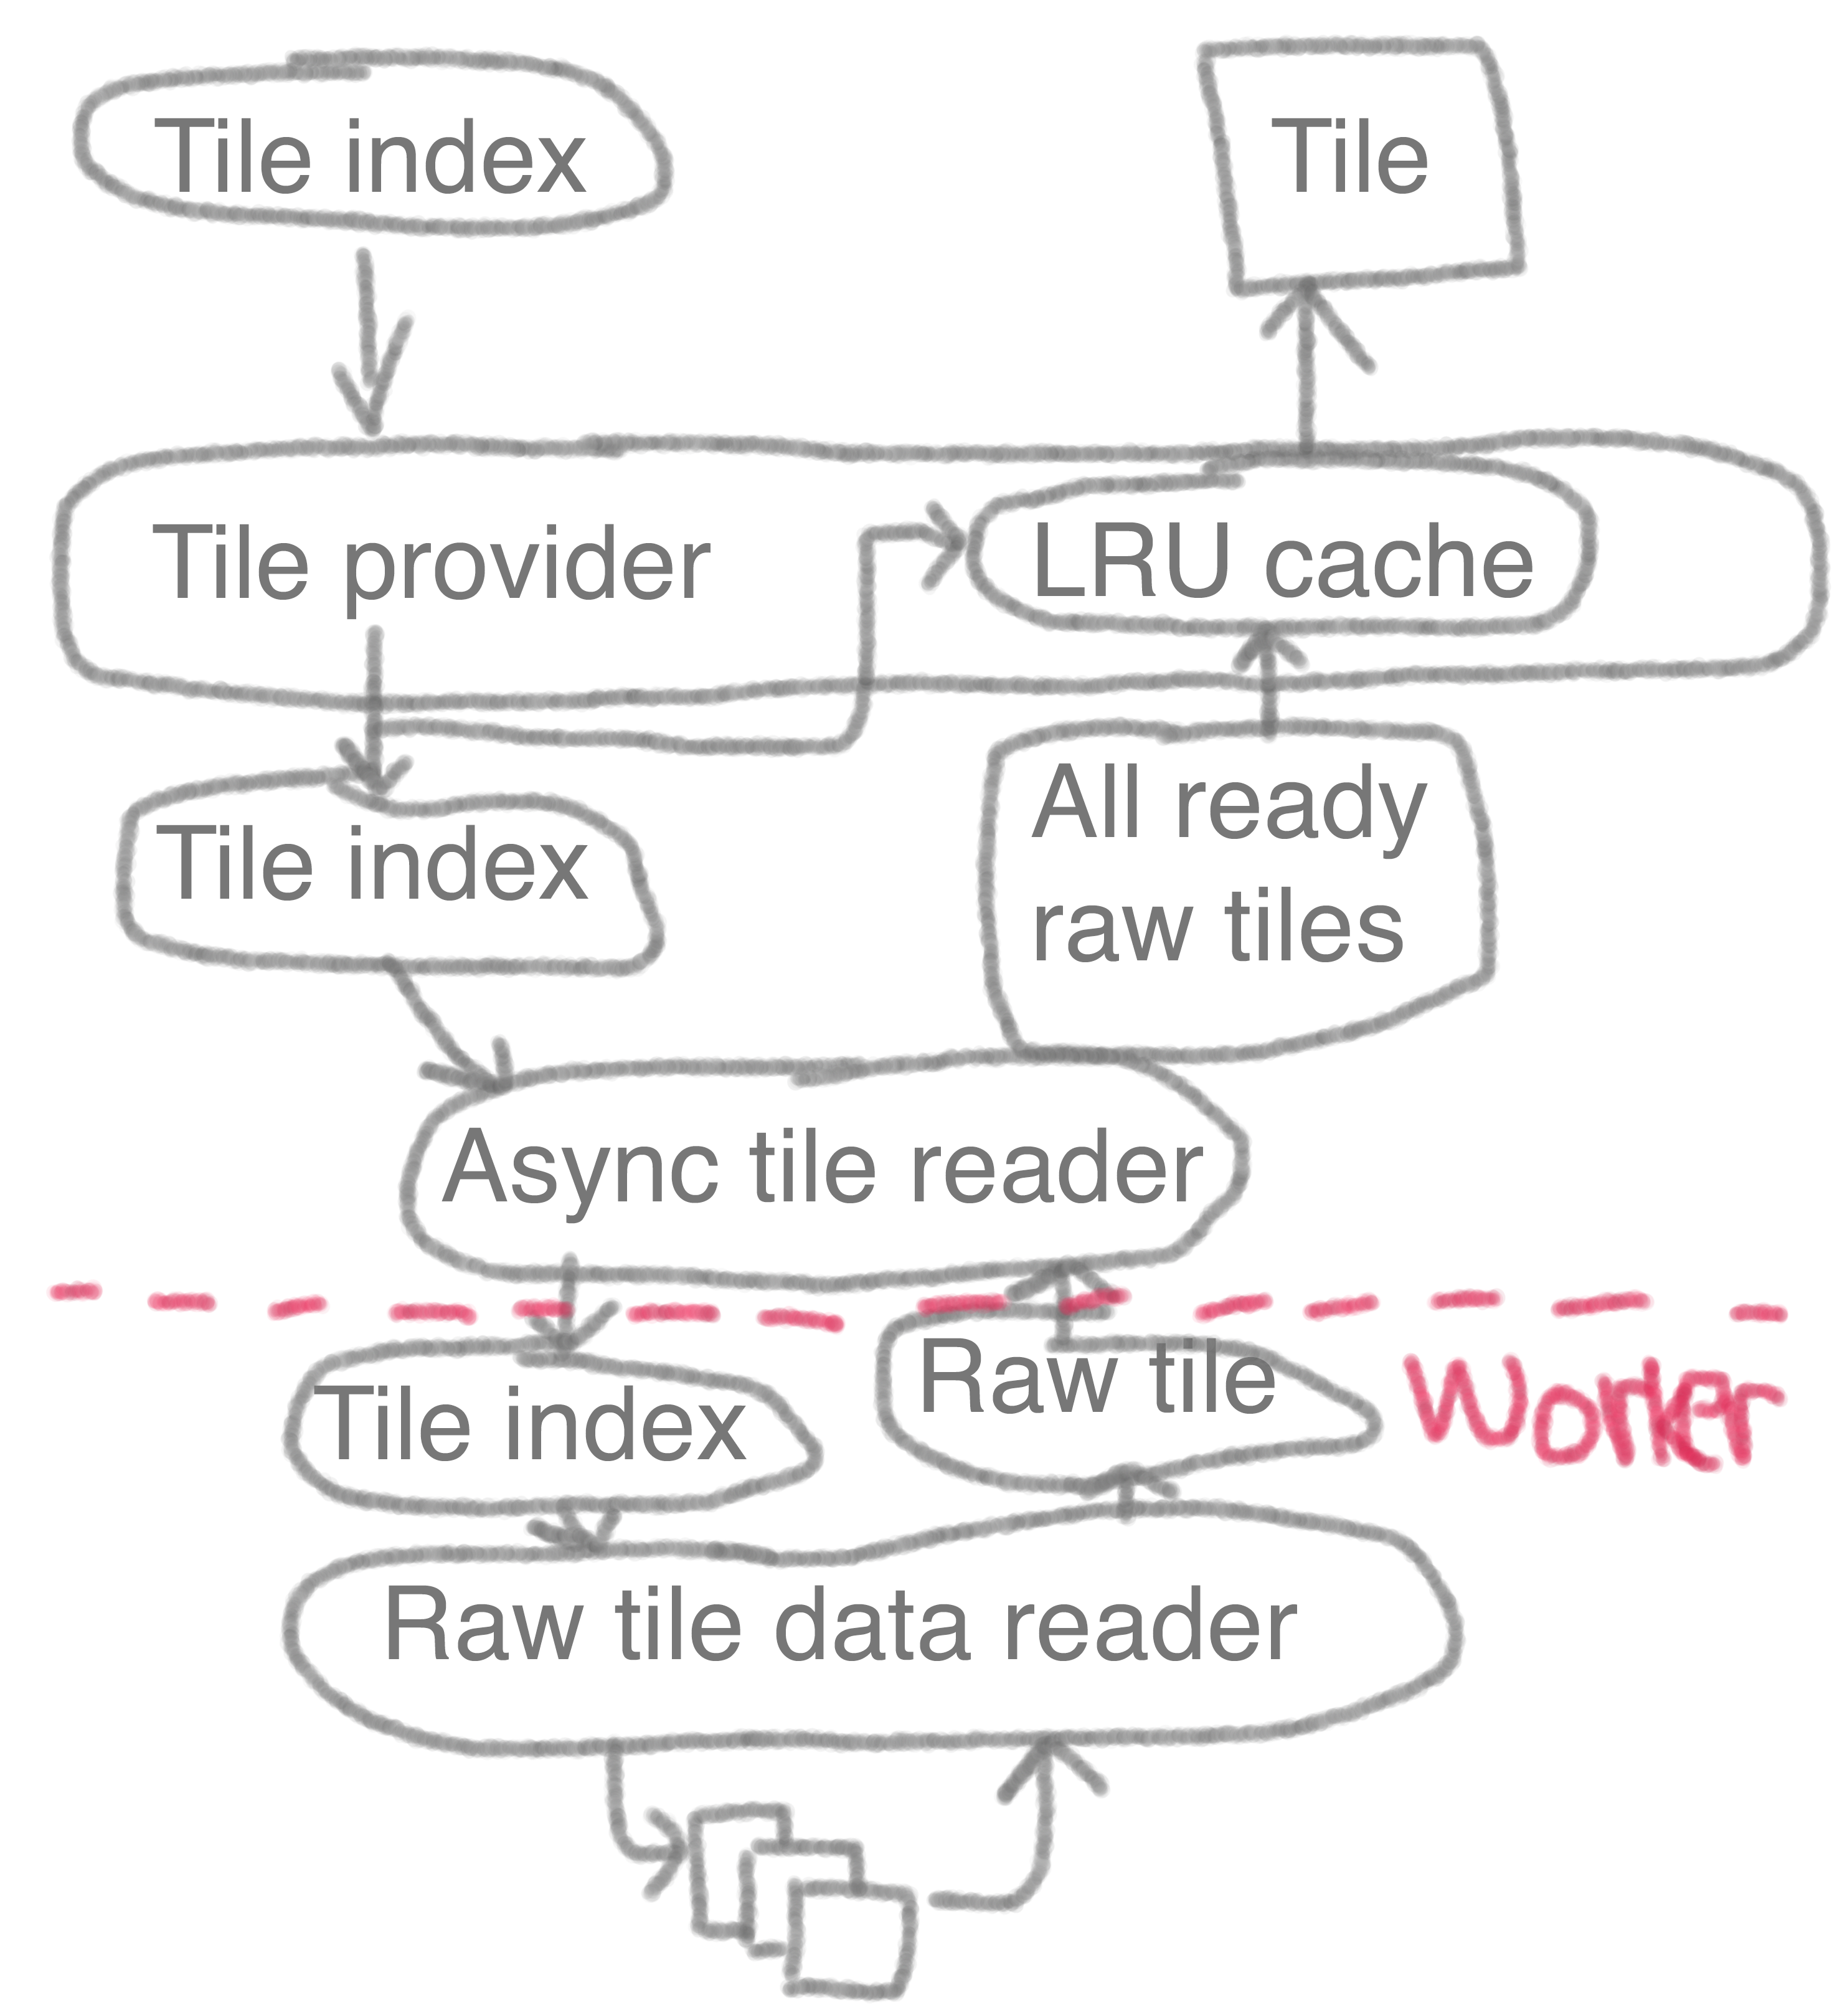
\includegraphics[width=0.5\textwidth]{figures/tile_pipeline.png}
%  \caption{Tile pipeline.}
%\end{figure}

%\kallecomment{Figure}

\subsubsection{Chunk Rendering} \label{sec:chunkrendering}

\begin{figure}
  \centering
    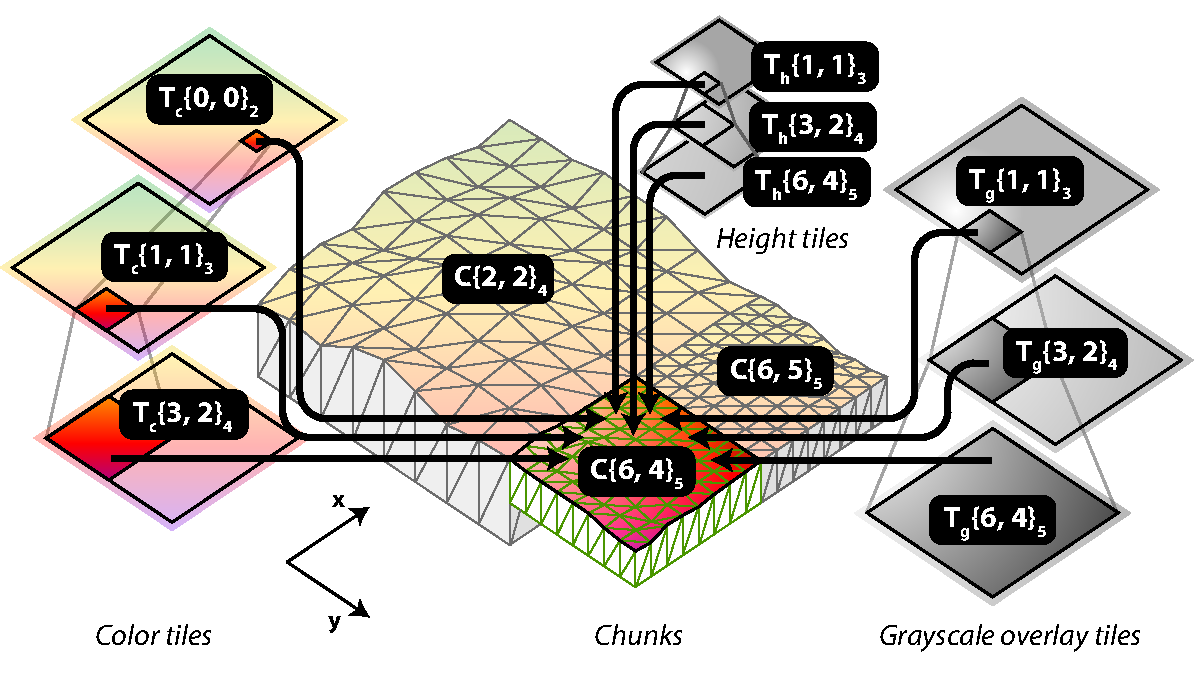
\includegraphics[width=1.0\linewidth]{figures/chunks-and-tiles4.pdf}
  \caption{Rendering a chunk $\textrm{C}\left\{ 6,4 \right\}_5$ by combining the information from a total of 9 tiles. For each of the three layer groups $\textrm{T}_\textrm{c}$~(color information), $\textrm{T}_\textrm{g}$~(overlay), and $\textrm{T}_\textrm{h}$~(height), the rendering of the main tile $\textrm{T}_\textrm{c}\left\{ 1,1 \right\}_3$,  $\textrm{T}_\textrm{g}\left\{ 3,2 \right\}_4$,  $\textrm{T}_\textrm{h}\left\{ 3,2 \right\}_4$ requires additional levels of detail to be loaded in order to provide an interpolation between layers.}\vspace*{-5mm}
  \label{fig:chunks-and-tiles}
\end{figure}


\begin{figure}[b]
  \centering
    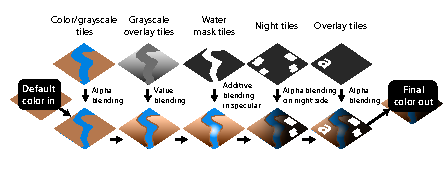
\includegraphics[width=1.0\linewidth]{figures/fragment-blending.pdf}
  \caption{Layer blending. Gray-scale overlays affects only the value component of the base color in HSV space. Water masks are used to change the specular reflection in the surface shading. Night tiles are particularly useful for Earth where cities illuminate the side that is not facing the sun. Geographical information can be added using overlay tiles.}
  \label{fig:fragpipe}
\end{figure}

Given a valid chunk tree, each chunk that is flagged as visible is rendered individually.
The geometry of the chunks is defined as a 2D regular skirted grid of vertices as seen in \fig{chunks-and-tiles}. This grid has a specific resolution in the size of the highest resolution height layer tiles. We avoid triangle decimation so that the same grid can be used for all chunk render calls. This makes our chunk tree representation light weight and dynamic as vertex offsetting is performed in the vertex shader.

%The downside of using a light weight chunk representation is that we are limited to the use of height mapping for vertex positioning which is done on the fly in the vertex shader.
%This, however saves us from preprocessing.
%This is useful since we can load height layers on demand and adjust each height layer's scaling factor if desired.
Each time a chunk needs to be rendered, all active layers will be queried for the most appropriate tiles.
%A tile can be transformed with a scale and an offset if it does not map 1:1 on to a chunk as seen in \fig{chunks-and-tiles}.
If the requested resolution level is not available lower levels will be used.
The renderer keep the two immediately lower resolution levels available as well such that appropriate blending can be applied.
%This is useful, not only for level blending (Section \ref{sec:fragment_blending}), but if a tile of a certain level is not available.
%the second best thing to do is to go down a detail level and fetch the available tiles of lower detail, adjusting the mapping on the chunk so that the corresponding geodetic area of the tile gets mapped on higher level chunks.


%\alexcomment{Kalle:  The vertices of a chunk need to be defined;  how is a chunk specified?  It was said earlier that the tree is lightweight}\plgrem{A chunk is light-weight as it does not hold any explicit geometry, it simply represents a region in the ellipsoid reference space. Geometry is generated on the fly by a tessellation shader using the height-map layer group. What is still unclear to me is how the LOD is determined for height-map and tessellation. The resolution is perhaps also flexible, or? I assume color and gray-scale layers need higher resolution than height-maps for a good visual appearance.}

To inversely project the vertices defining the chunk grid, from georeferenced coordinates to the model space of the globe, we employ two different types of rendering techniques to account for both accuracy and precision.

\paragraph{Model-space rendering}

Using the inverse projection $P^{-1}(\phi,\theta)$, vertices of a given chunk are unprojected from the georeferenced projection to the Cartesian model space of the globe.

This unprojection is performed in single precision on the GPU and results in the chunk being accurately mapped to the curvature of the reference ellipsoid.

\paragraph{Camera-space rendering}

The same inverse projection can be performed in double precision on the CPU for the four corner points of the chunk.
These points are then transformed to camera space in double precision where they are then casted to single precision and uploaded to the GPU.
Now the rest of the vertices representing the chunk can be bilinearly interpolated for the chunk to be mapped on to the reference ellipsoid.

This method results in high precision rendering due to the origin practically being moved to the center of the camera.
The accuracy is lower however since the chunks are approximated as flat surfaces as a result of the bilinear interpolation.

\paragraph{Combined model- and camera-space rendering}

To achieve both the accuracy required for the curvature and the precision required for rendering small chunks close to the camera, we simply use a cutoff level $k$ where chunks below it that are big, and need to be curved, are rendered with the model space method as illustrated in \fig{chunkproc}.
All smaller chunks, which are better approximated as flat surfaces, are rendered with the camera space method since their vertical error metric, due to curvature, is smaller.

For example, a cutoff level of $k = 10$ for Mars lead to a maximum vertical error of $e = r - r \cos{(360/(2^{k + 1}))} \approx 16$ meters with $r=3 390$ km.
With chunks of width $r \sin{(360 / (2^{10 + 1})} / 2 \approx 296$ km, 16 meters become insignificant and as the chunks split, higher levels will lead to smaller error.

\paragraph{Fragment blending} \label{sec:fragment_blending}

To account for versatility and seamless level switching %\cite[p. 450]{cozzi20113d}
we perform three different types of fragment blending:

\noindent\textbf{Layer group blending} is performed so that many different layer groups can be combined together.
In a pipeline fashion, each active layer group is sampled and composited to get the final color, as shown in \fig{fragpipe}.
One important example is the use of gray-scale overlays on top of color layers.
The grayscale overlay layer group is used to sample the underlying color (hue and saturation) and setting the intensity (value) according to the value of the gray-scale overlays.
Another example is the night layers which will be sampled on the night side of the globe, if any are activated.

\noindent\textbf{Layer blending} is performed so that many layers in the same layer group can be rendered together. Layers can be manually ordered and combined using a per-layer opacity parameter. Furthermore, using alpha blending, local high-resolution patches can be rendered on top of other datasets with lower resolution.

\noindent\textbf{Level blending} is performed to achieve smooth transitions between levels, to avoid popping artifacts. It differs from Ulrich's time-varying blending \cite{ulrich2002rendering} in that
we calculate an interpolation parameter for each fragment depending on its distance to the camera.
This interpolation parameter is used to interpolate between the tile of the current chunk level and the corresponding tiles of the two immediately lower-level tiles, see Figure \ref{fig:chunks-and-tiles}. The interpolation parameter is calculated according to \fig{switchingblending}.

\begin{figure}
    \centering
    \begin{subfigure}[tb]{0.24\textwidth}
    	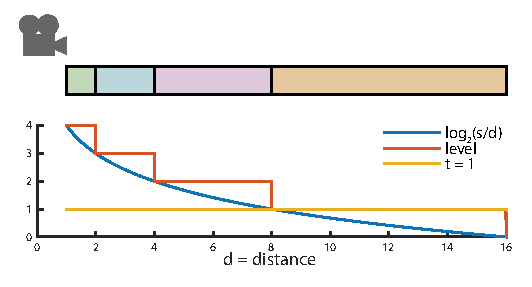
\includegraphics[width=\textwidth]{figures/blending1b.pdf}
	\caption{Blending disabled.\\ Only need of sampling one tile.}
    \end{subfigure}
    \begin{subfigure}[tb]{0.24\textwidth}
    	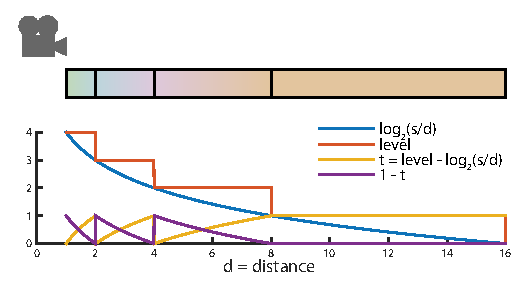
\includegraphics[width=\textwidth]{figures/blending2b.pdf}
	\caption{Blending enabled.\\Two tiles or more are required.}
    \end{subfigure}
    \caption{Blending on a per fragment basis. The level interpolation parameter $t$ is used to calculate level weights $w_1 = 1-t$ and $w_2 = t$. The level weights are used to combine sampling from high level tiles with low level tiles. In practice we can use up to three tiles of different level, in the figure the concept is illustrated using two tiles.}  \vspace{-4mm}
    \label{fig:switchingblending}
\end{figure}

We use shader preprocessing to opt out any unused blending option.
As soon as a layer is activated, or deactivated or if blending is enabled or disabled we recompile the fragment shader to only sample textures that contribute to the final color of the chunk.

\subsubsection{Time Varying Datasets}

NA specific, \emph{temporal} tile provider has the ability to create its own tile providers, where each one corresponds to its own time interval.
When the global time of the software gets to a different time interval, the temporal tile provider will start instantiating tile reading calls to a different tile provider corresponding to that time interval.
This can undoubtedly lead to a lot of reading within a short amount of time so memory buffering becomes important for temporal datasets.
In our implementation, memory buffering is a manual process of browsing the wanted data to cache it for later time scrubbing.

\subsection{Multi Display Systems Rendering} \label{sec:multidisplaysystems}

The OpenSpace software uses the cluster rendering software package Simple Graphics Cluster Toolkit (SGCT)~\cite{sgct} which supports image warping and blending for projection on dome displays and other clustered environments using several rendering machines.
Synchronization across rendering nodes is based on GenLocking at the graphics hardware level and SGCT furthermore provides support for synchronization of selected application data at frame rendering level, ensuring that all nodes in the cluster renders a given frame with the same camera configuration.
Tile loading and chunk LOD selection is autonomous on each node, which visually can result in minor differences in the projector blending regions. However, due to the use of camera direction independent chunk selection algorithms, each rendering node will request the right tiles to be used across projector edges. The loading time can differ however since each node uses their own tile reading request queue.
This is normally not an issue as navigation and movement in dome setting need to be slow to moderate to avoid cyber sickness.

Figure \ref{fig:power_wall} shows an example of our software used in a multi display system known as a power wall.

\begin{figure}
    \centering
    	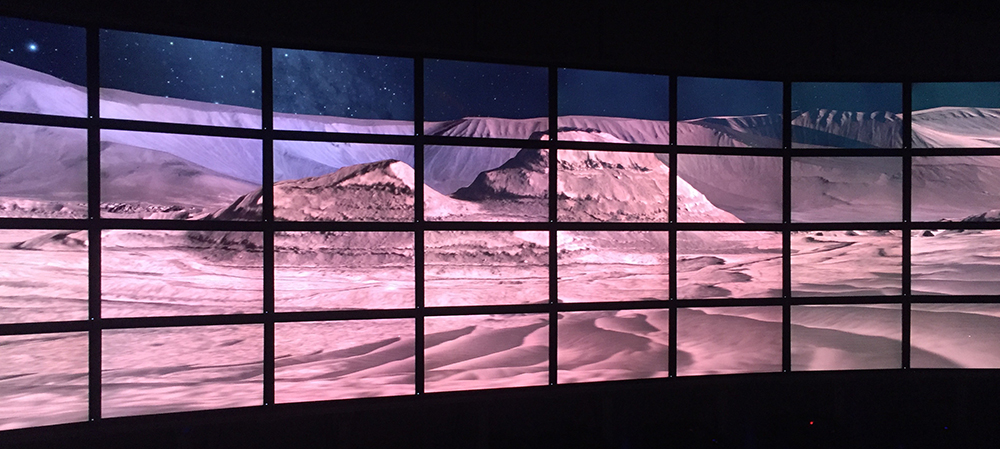
\includegraphics[width=1.0\linewidth]{figures/power_wall.jpg}
        \caption{Browsing the surface of Mars in a clustered environment rendering on the power wall at the University of Utah. The system uses eight rendering nodes, each connected to four screens.}  \vspace{-4mm}
    \label{fig:power_wall}
\end{figure}

\section{Results}
%\anderscomment{We have to make sure that this section doesn't become a repeat of the application scenarios section with some more details added.
%}

Here we present our results exemplified by the three application scenarios introduced in Section \ref{sec:scenarios}. We perform a globe browsing descent towards the surface of mars measuring frame time and the size of the chunk tree. We also show how the Earth can be rendered with temporally varying textures of high resolution. Finally exemplify how our application is used to communicate the data acquisition process of the New Horizons fly by of the Pluto system.

\subsection{Globe Browsing on Mars}


\begin{figure*}
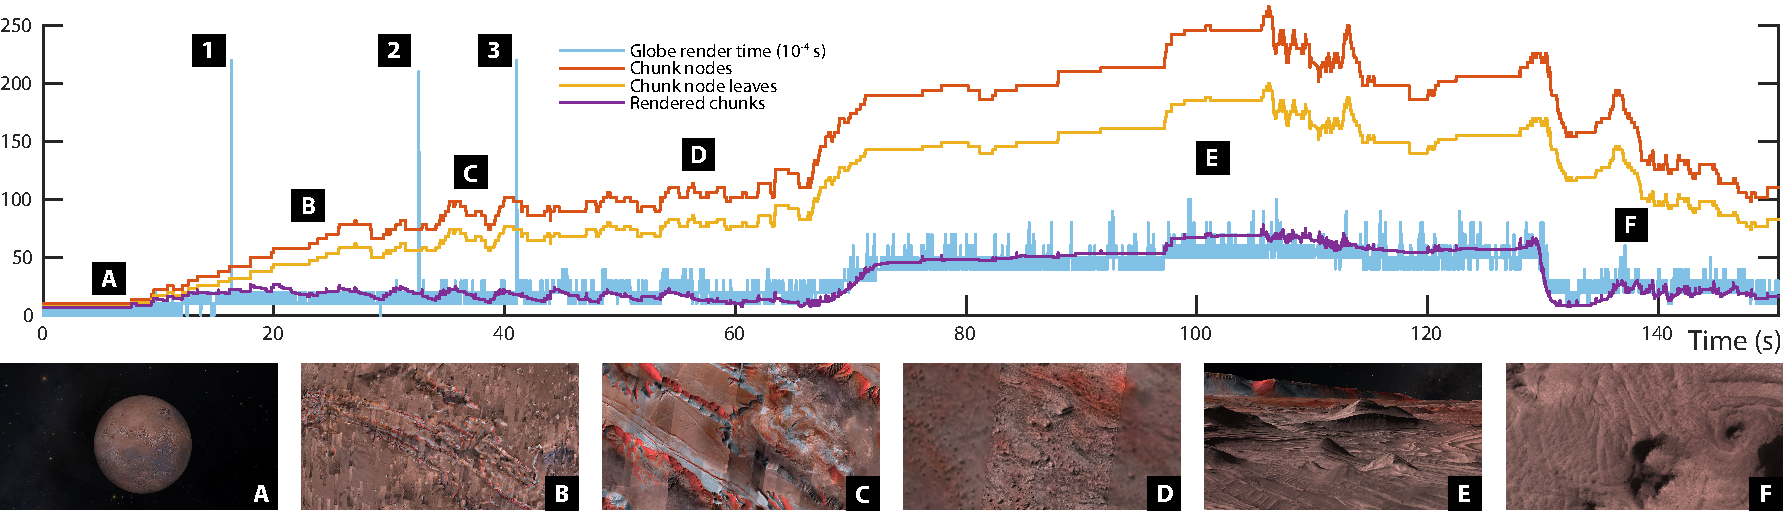
\includegraphics[width=\linewidth]{figures/marsbrowsing5_compressed.pdf}
\caption{Globe browsing session on Mars: top graph shows size of the chunk tree along with the total render time. 1) Global CTX Mosaic enabled, 2) Local CTX patch enabled, 3) Local HiRISE patch enabled. A) Camera approaches Mars, B) Valles Marineris, C) West Candor Chasma, D) Layered rock outcrops in South West Candor Chasma, E) Camera tilted up, F) Camera rotated and then tilted down.}  \vspace{-2mm}
\label{fig:globebrowsingmars}
\end{figure*}

We chose Mars as one of the application scenarios due to the availability of high resolution images and can thus demonstrate the ability of the system to handle large scale differences.

In our test session, illustrated in Figure \ref{fig:globebrowsingmars} Mars is rendered using the global Viking Color mosaic 2.1 as a base color layer.
The global MOLA height layer is used as a base DTM for terrain information.
Furthermore, in order to achieve more detail, we include the Global CTX mosaic, as well as local patches that contain DTM and textures from the CTX and HiRISE camera.

The computer used for the evaluation is a HP Z420 Workstation with an Intel Xenon CPU E5-1620 3.60 GHz 4 Core processor, an NVIDIA GeForce GTX 780 GPU and 8192 MB RAM memory.

\fig{globebrowsingmars} provides important insights in how the frame time depends on the loading of data and the size of the chunk tree.
When activating new layers, the frame time increases.
By descending closer to the surface, more of the chunk tree have to be traversed but leaves the number of rendered chunks constant due to the two culling methods.
Tilting the camera leads to initialization of tile reading calls which in turn causes the chunk tree to grow over time as more tiles become available.
Following point E, the camera is rotated thus decreasing the chunk tree due to unavailable tile data in areas previously invisible to the camera.
As soon as the data is read and available, the chunk tree grows since it no longer is limited by the unavailable data.
As soon as the camera is tilted down again, the number of rendered chunks decrease.

\iffalse{}

\begin{figure}
    \centering
    \begin{subfigure}[tb]{0.24\textwidth}
    	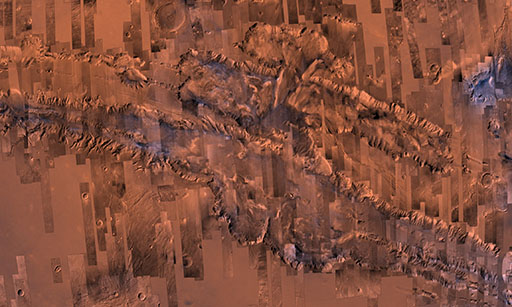
\includegraphics[width=\textwidth]{figures/valles_marineris3.jpg}
	\caption{Valles Marineris, Global CTX mosaic over Viking color.}
    \end{subfigure}
    \begin{subfigure}[tb]{0.24\textwidth}
    	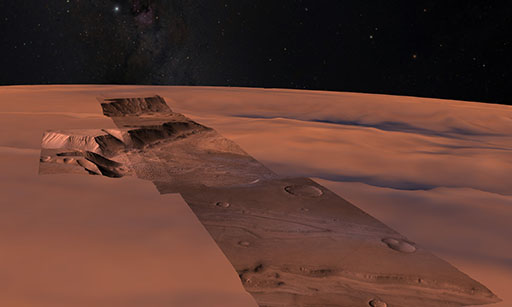
\includegraphics[width=\textwidth]{figures/west_candor_chasma1.jpg}
	\caption{Local CTX patch and corresponding DTM generated from stereo pairs.}
    \end{subfigure}
    \begin{subfigure}[tb]{0.24\textwidth}
    	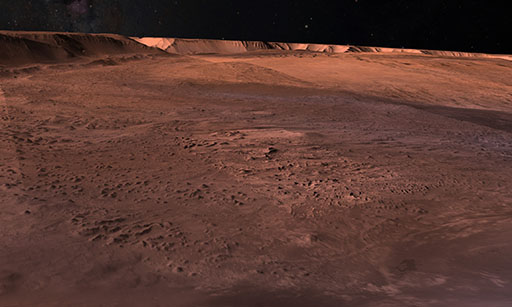
\includegraphics[width=\textwidth]{figures/west_candor_chasma2.jpg}
	\caption{A HiRISE patch inside the area of the CTX patch.}
    \end{subfigure}
    \begin{subfigure}[tb]{0.24\textwidth}
    	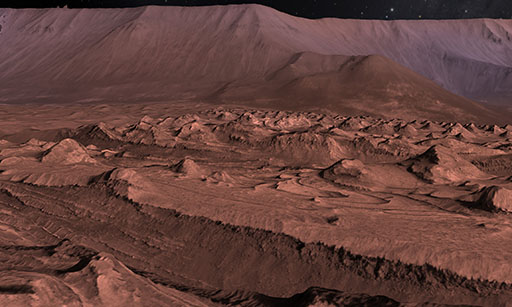
\includegraphics[width=\textwidth]{figures/west_candor_chasma3.jpg}
	\caption{Close up detail of the HiRISE patch. Camera is now roughly 50 meters from the surface.}
    \end{subfigure}
    \caption{}
    \label{fig:globebrowsingmars}
\end{figure}


\fig{lodcomp} shows the difference in number of chunks rendered depending on the choice of chunk selection procedure.

\begin{figure}[h]
\centering
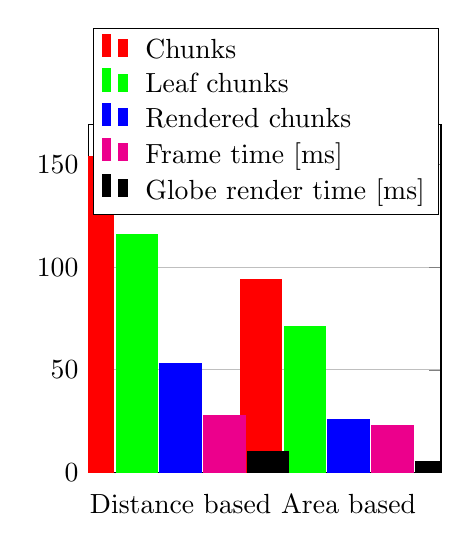
\begin{tikzpicture}
    \begin{axis}[
        width  = 0.5*\textwidth,
        height = 6cm,
        major x tick style = transparent,
        ybar=2*\pgflinewidth,
        bar width=15pt,
        ymajorgrids = true,
        ylabel = {},
        symbolic x coords={Distance based, Area based},
        xtick = data,
        scaled y ticks = false,
        enlarge x limits=0.55,
        ymin=0,
        legend cell align=left,
        legend style={
                at={(0.995, 0.74)},
                anchor=south east,
                column sep=1ex
        }
    ] 

      \addplot[style={red,fill=red,mark=none}]
        coordinates { (Distance based, 154) (Area based, 94) };

      \addplot[style={green,fill=green,mark=none}]
        coordinates { (Distance based, 116) (Area based, 71) };

      \addplot[style={blue,fill=blue,mark=none}]
        coordinates { (Distance based, 53) (Area based, 26) };

      \addplot[style={magenta,fill=magenta,mark=none}]
        coordinates { (Distance based, 28) (Area based, 23) };

      \addplot[style={black,fill=black,mark=none}]
        coordinates { (Distance based, 10) (Area based, 5.6) };

      \legend{Chunks, Leaf chunks, Rendered chunks, Frame time [ms], Globe render time [ms]}

    \end{axis}
\end{tikzpicture}
\caption{Comparison of distance based and area based chunk selection}
\label{fig:lodcomp}
\end{figure}

\fi{}

To further show how the different data products contribute in building the chunk tree, \fig{load-times} illustrates the loading time for each of the Mars datasets when the camera is positioned 50\,m above ground in the area of the HiRISE patch.
The number of rendered chunks is directly dependent on the data source used due to the chunk level being limited by the availability of data.
Hence, the final number of chunks differs depending on the data source. 
This scenario combines data sources stored on local WMS servers (CTX Mosaic and MOLA) and local patches stored on hard disk (HiRISE) and there is no significant difference between the loading times of the two.

\begin{figure}
  \centering
    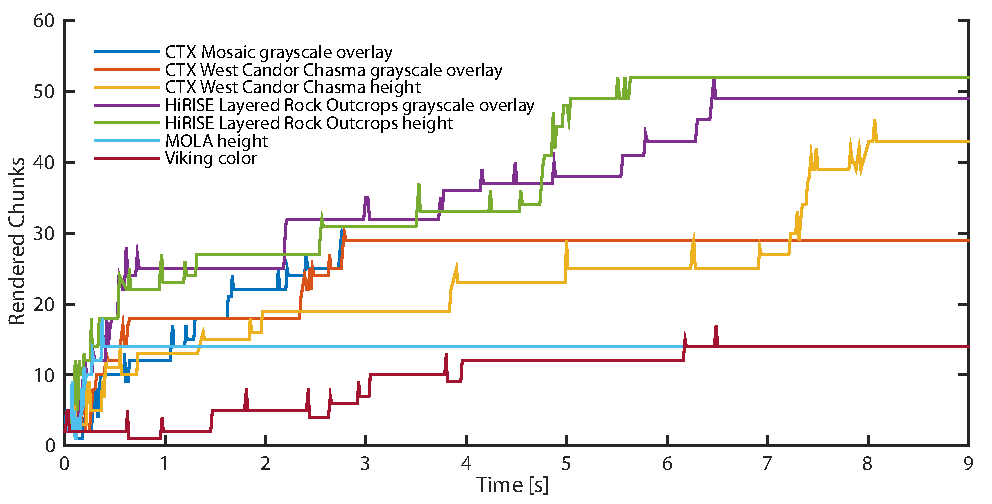
\includegraphics[width=1.0\linewidth]{figures/load_times.pdf}
  \caption{Loading times of different data sources illustrated by the number of rendered chunks over time. Each recording is performed separately by enabling the layer when the camera is 50 meters from the ground facing the horizon. Depending on the data source, the resulting number of rendered chunks differs.}  \vspace*{-4mm}
  \label{fig:load-times}
  \end{figure}

\begin{figure}
    \centering
    	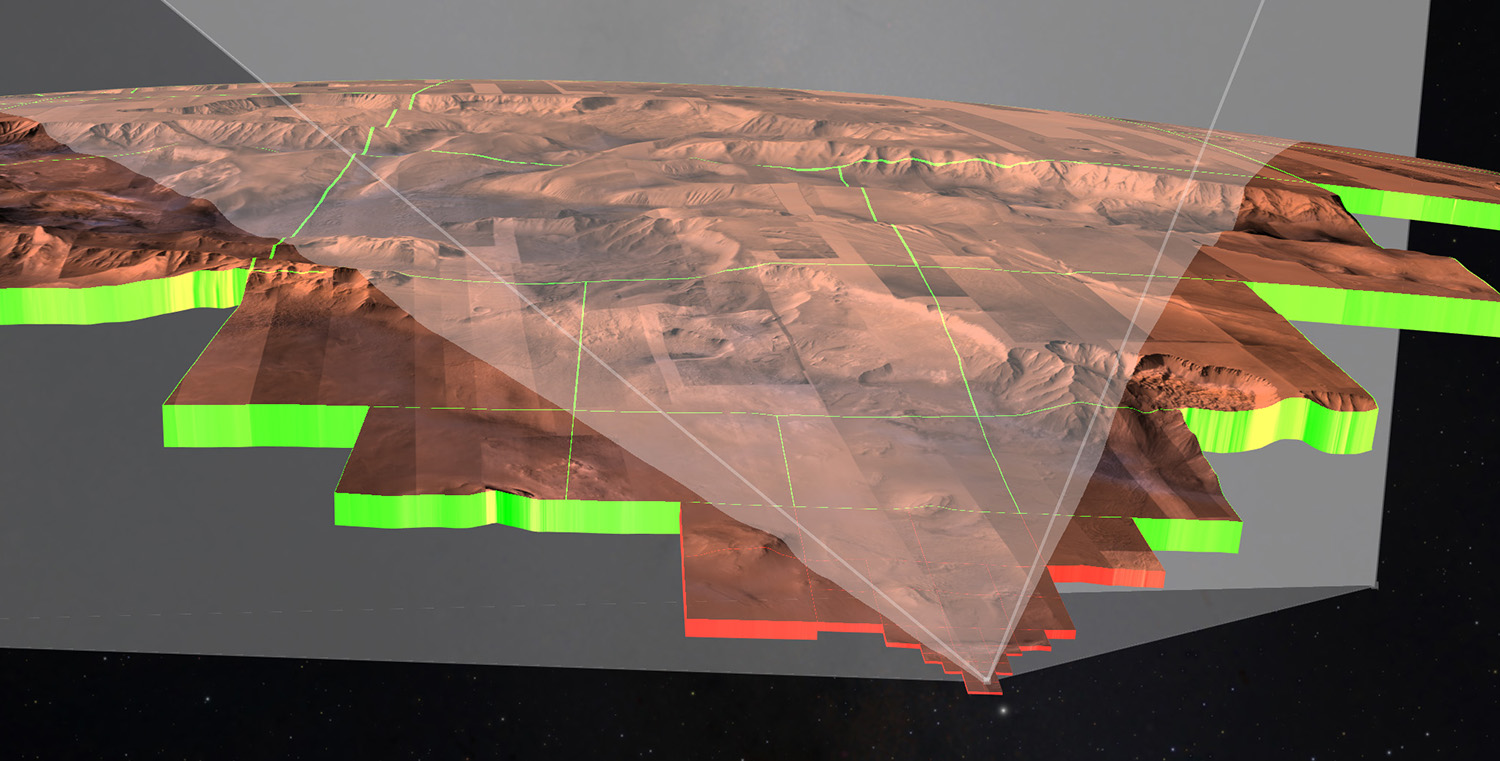
\includegraphics[width=1.0\linewidth]{figures/frustum_mars.jpg}
        \caption{Camera frustum and horizon culling illustrated by showing the cameras view. Model space rendering of chunks (green) is performed when the level is higher or equal to 10. Camera space rendering of chunks (ref) is performed for all higher levels.}\vspace*{-4mm}
    \label{fig:frustum_mars}
\end{figure}

The Mars globe browsing sessions have been used in a large number of public presentations as a means to explain the history of Mars, and the ability to contextualize and explain events pertaining to the rovers on the surface.
These public education events using the available Mars data has been ongoing for the past year and have reached thousands of people using the multi display systems as described in Section~\ref{sec:multidisplaysystems}.

\subsection{Temporal Datasets on Earth}
In addition to the ongoing public events using the high-resolution Mars data from the previous section, a global, public event is planned on April 22nd coinciding with Earth Day, that will celebrate the knowledge about our planet and make this data available to the general public.
This event will connect five locations around the world and provide a video stream of Earth scientists utilizing this system to explain the complex temporal behaviors of the Earth and how we achieved these measurements.
The scientists will be located at the Hayden planetarium in New York, but will be interacting with every audience member around the world.
Utilizing the presented system, they scientists will be able to place their own data and measurements into their accurate location, and thus context, in order to communicate their data to the public.

\fig{temporal_earth} (top row) contains images from the time-varying VIIRS datasets over a few days, showing the location and movement of clouds on Earth. The bottom row shows the local fluctuations of the sea surface temperate over a few months. Both datasets are provided by NASA GIBS.
By combining these data sources it becomes possible to contextualize, for example, the creation of a hurricane in the Atlantic by showing the sudden temperature change that coincide with the generation of a large cloud area.

As the \emph{Aqua} and \emph{Terra} satellites have been collecting data for the last 17 years, it is further possible to show the long term evolution of individual locations on Earth, such as the drying of Lake Mead.
Showing these large scale changes at a variety of locations around Earth plays an important role in educating the general public about the impact of human society on everyone's planet.

\begin{figure}
    \centering
    \begin{subfigure}[tb]{0.32\linewidth}
    	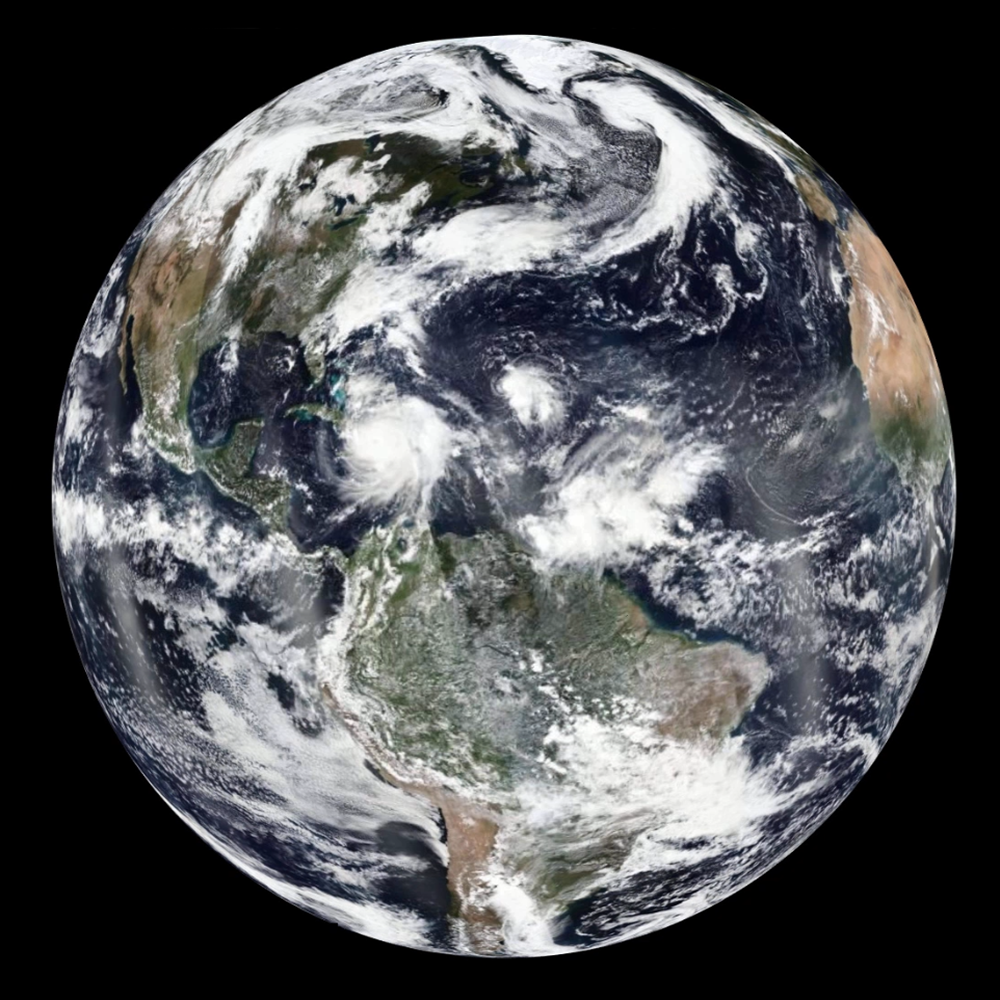
\includegraphics[width=\textwidth]{earth_temporal/earth_temporal_viirs1.png}
	\end{subfigure}
    \begin{subfigure}[tb]{0.32\linewidth}
    	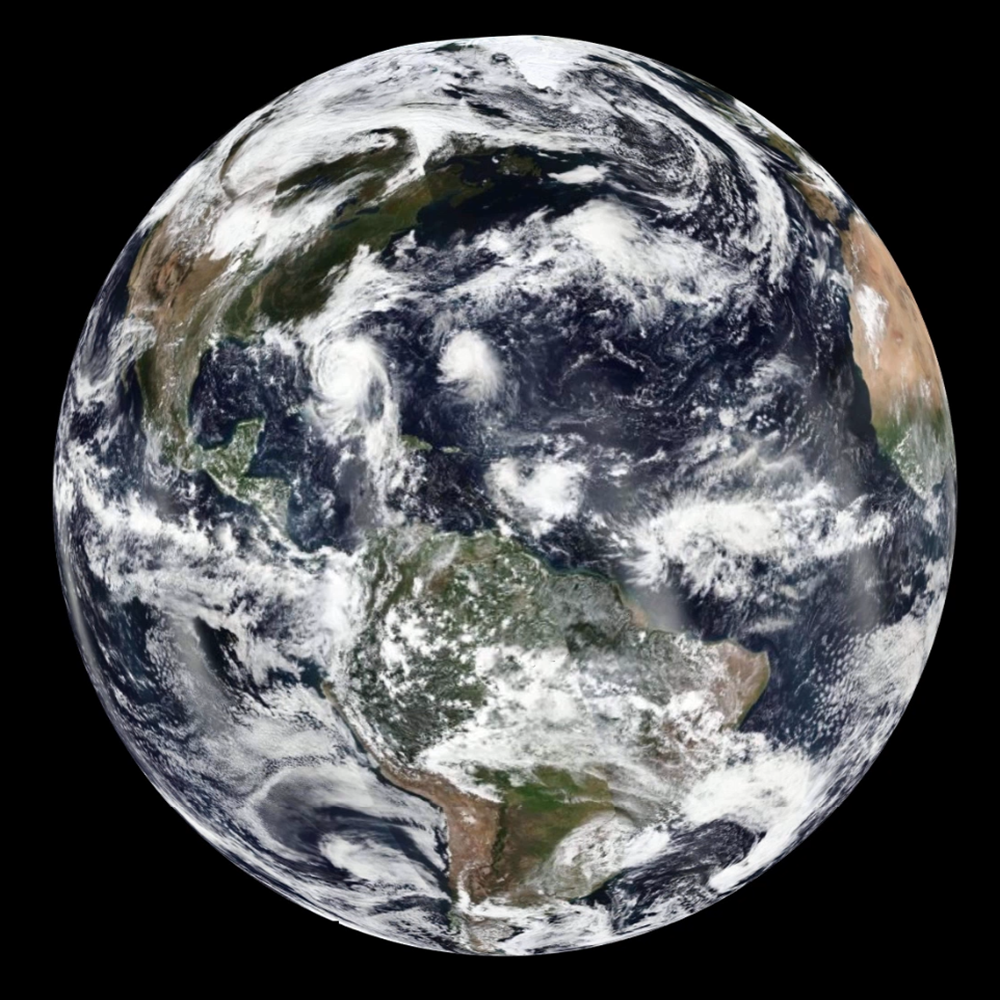
\includegraphics[width=\textwidth]{earth_temporal/earth_temporal_viirs2.png}
	\end{subfigure}
    \begin{subfigure}[tb]{0.32\linewidth}
    	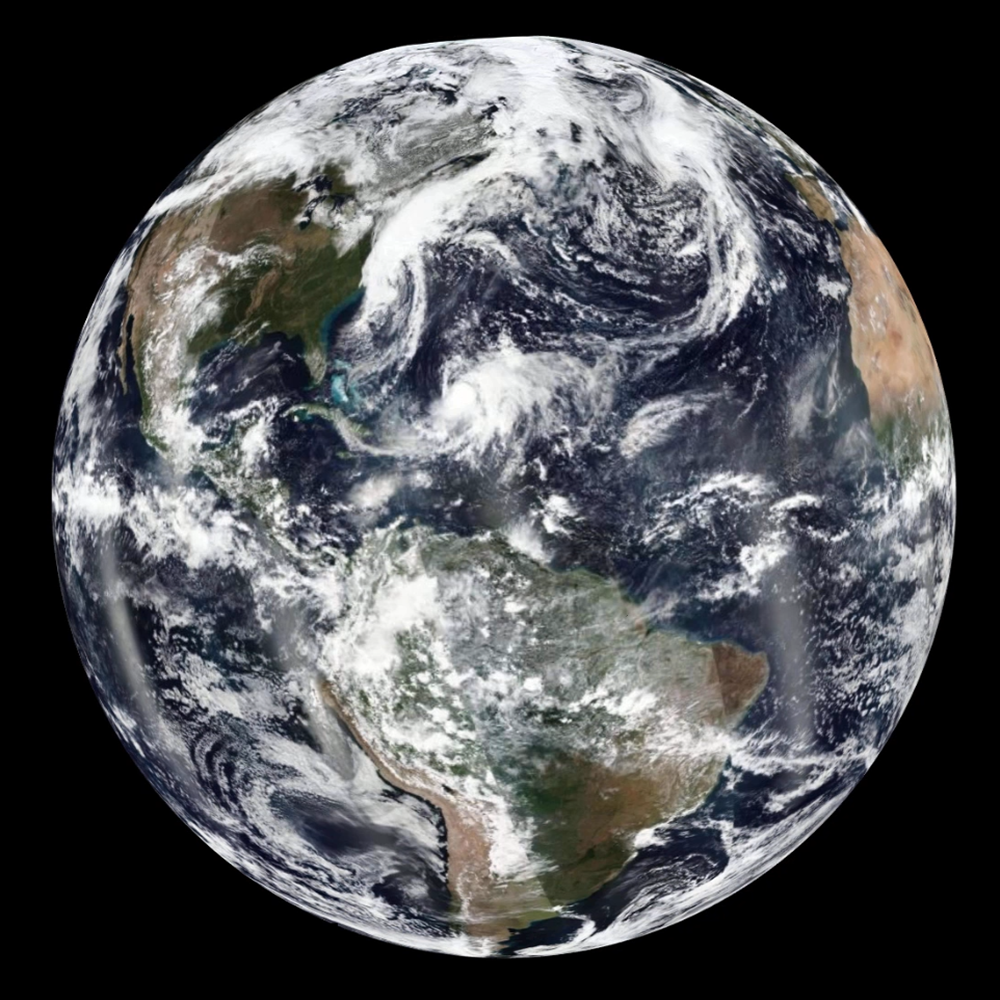
\includegraphics[width=\textwidth]{earth_temporal/earth_temporal_viirs3.png}
	\end{subfigure}

	\begin{subfigure}[tb]{0.32\linewidth}
    	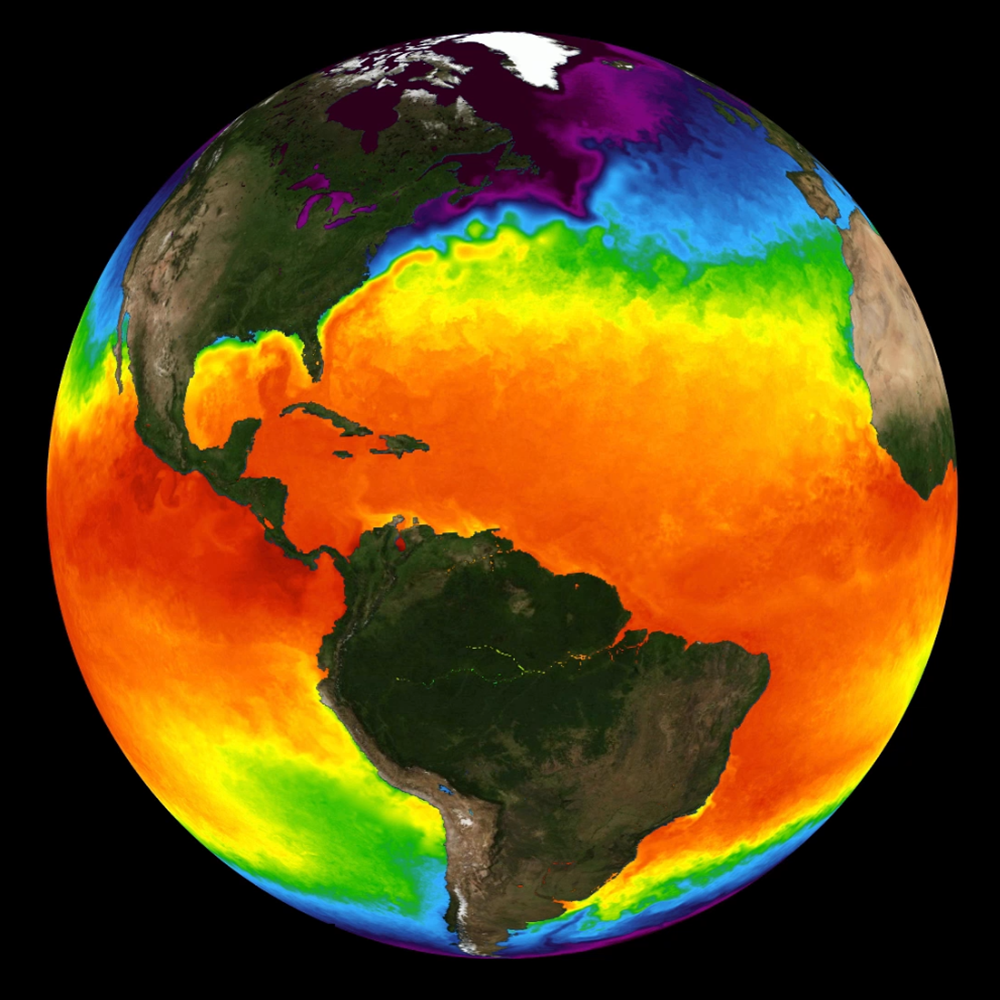
\includegraphics[width=\textwidth]{earth_temporal/earth_temporal_sea_surface1.png}
	\end{subfigure}
    \begin{subfigure}[tb]{0.32\linewidth}
    	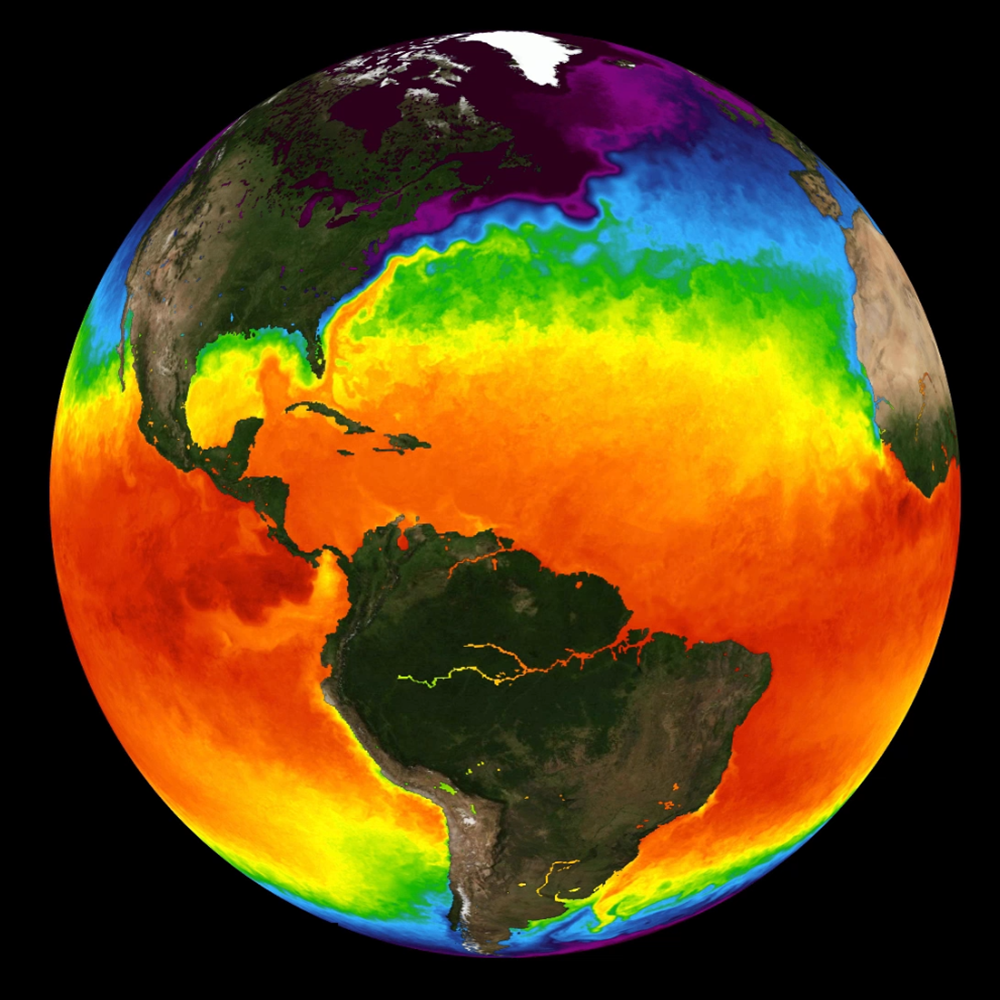
\includegraphics[width=\textwidth]{earth_temporal/earth_temporal_sea_surface2.png}
	\end{subfigure}
    \begin{subfigure}[tb]{0.32\linewidth}
    	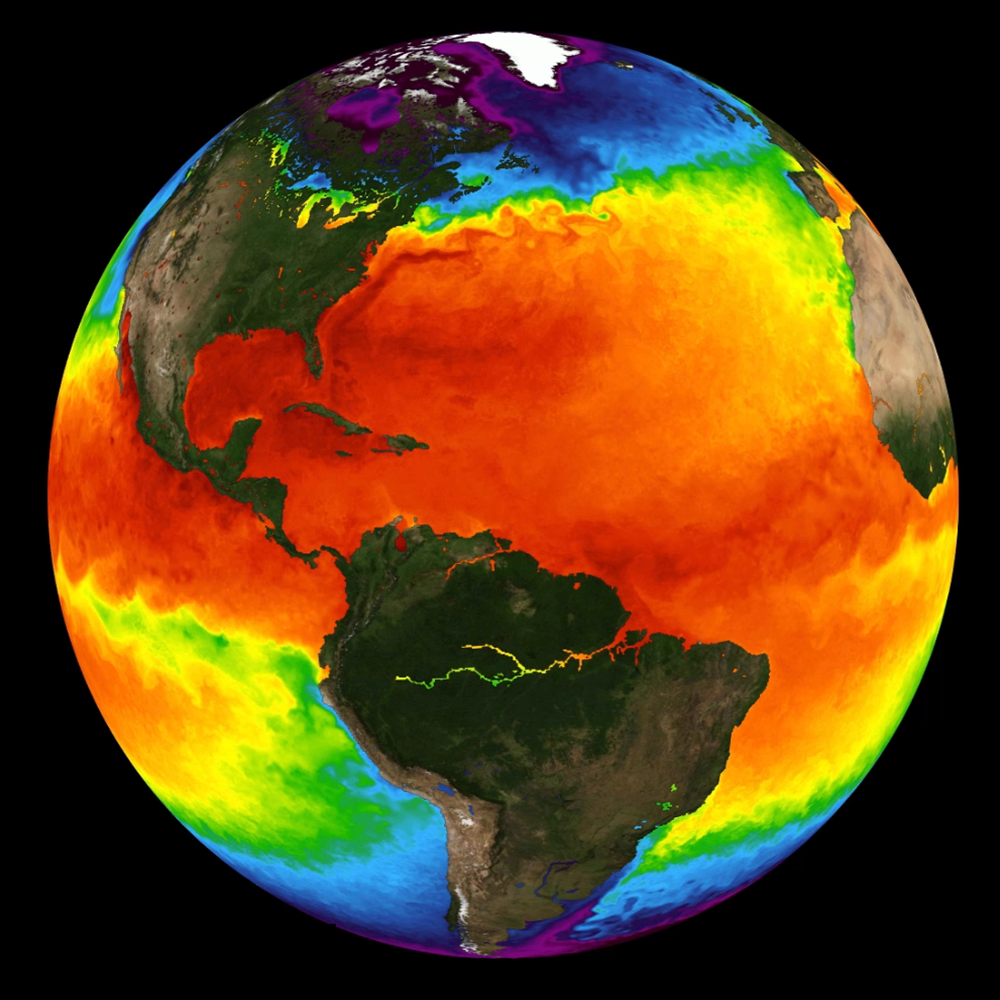
\includegraphics[width=\textwidth]{earth_temporal/earth_temporal_sea_surface3.png}
	\end{subfigure}
    \caption{These images show the temporal behavior of Earth's cloud formations (top row) from the Suomi NNP satellite's VIIRS instrument over the course of a week. The sea surface temperature (bottom row) is retrieved over the course of three months from the Group for High-Resolution Sea Surface Temperature (GHRSST).}  \vspace{-4mm}
    \label{fig:temporal_earth}
\end{figure}


\subsection{Visualizing Acquisition on Pluto}
NASA's New Horizons mission flew by the Pluto system on July 14th, 2015 and took measurements with its seven instruments.
Of special interest are the LORRI and RALPH instruments, that provided images of Pluto and its moons' surfaces, as well as REX, measuring Pluto's atmosphere, see Section~\ref{sec:scenario:pluto} for more information on the instruments.
In our system, the images are projected using the method described in Section~\ref{sec:imageprojection}.
The user can follow the progression of the spacecraft over time and seeing the instrument activities.
In addition to visualization of the instrument frustrum and projected images, the measurement times for all instruments are presented to the user. 

This mission visualization was presented to about 2500 people during a public, global event in which 13 different locations participated.
During a 2\,h live show, which coincided with New Horizons closest approach to Pluto, experts on the mission team explained details of the desired outcome using \emph{OpenSpace} as the source of the contextualization for these informations, see \fig{frustum_mars}.
In addition to the live audience in the participating locations, a video stream of the event was available on the web. This was also later provided as a video-on-demand, called ``Breakfast at Pluto''.
The event is described in the SciVis Poster on public dissemination of space mission profiles by Bock~\etal~\cite{Bock_2015}.
Some initial results from the New Horizons mission are given by Stern~\etal~\cite{stern2015pluto}.
The visualizations have also been used in several post flyby events showing the incremental update of our knowledge about this object to the general public.

\begin{figure}[b]
\vspace*{-5mm}
    \centering
    	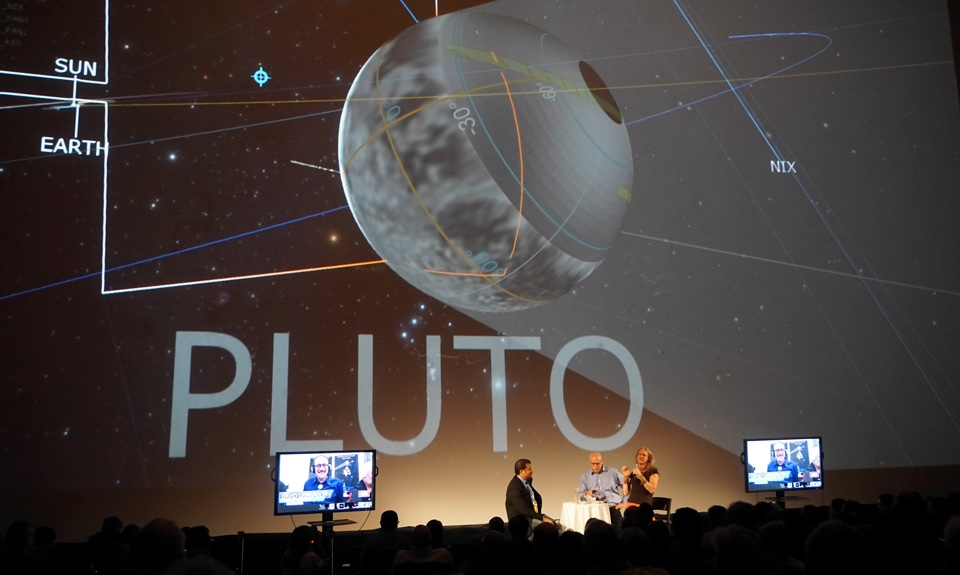
\includegraphics[width=0.5\textwidth]{figures/breakfast.jpg}
        \caption{OpenSpace was used to visualize how New Horizons captured images of Pluto on July 14th, 2015. Sites from all over the world connected in a live event during the flyby. The image shows the New York site with host Neil deGrasse Tyson.}\vspace*{-2mm}
    \label{fig:frustum_mars}
\end{figure}


%\alexcomment{Previous New Horizons text:}
%One of the main science instruments that is used on spacecraft are digital cameras that take images. In order to present these images to the audience, they are projected onto the target body using projective texturing as described by Everitt~\etal~\cite{Everitt:2001tg}. As images are mostly acquired in quick succession, this leads to a mosaic covering of the target, as was done on by the New Horizons mission on Jupiter in 2007 (see \fig{jupiter}). In the cases where the whole image does not cover a body, a virtual image plane is added that contains the remainder of the image (see \fig{pluto}).

%NASA's mission will fly by the Pluto system on July 14th, 2015 and will take measurements with its seven instruments. Of special interest are the LORRI and RALPH instruments, that will take images of Pluto's and Charon's surface, as well as REX that will take radio measurements of Pluto's atmosphere (see \fig{radio}). In our system, the images are projected using the method described above and the REX occultation measurements are represented by a line connecting the spacecraft and Earth. The measurement times for all instruments are presented to the user, but not all instruments have a direct visual mapping, for example the SWAP instrument measures solar wind density values. The components for this mission were shown at the American Museum of Natural History's Evening for Educators event on May 14th that part of the Pluto Palooza event series. In addition, the July 14th fly-by will be shown at various locations around the globe.

%As one of the major motivations for developing this method, spacecraft are inherently small objects that need to be visualized precisely with respect to an object, mostly planets, that they are inspecting.
%One example is shown in \fig{teaser} where the New Horizons spacecraft is shown at 80\,Mm distance to Pluto and around $6 \cdot 10^{12}$\,m away from the Sun.
%As described in Section~\ref{sec:floating-point-numbers}, floating point numbers only have a precision of about 300\,km at the distance of Pluto, which would make a traditional approach infeasible. With our method, however, it is possible to show the entire mission with the required precision.


%\anderscomment{This paragraph can go if we need to save space}
Space missions, such as \emph{New Horizons} or \emph{Cassini}, are very expensive endeavors carried out in the public interest. These missions are planned years in advance in order to maximize the scientific output they produce. Due to this streamlining and the lack of available tools for the general public, the spacecraft's actions during the scientific exploration can be difficult to understand and communicate. The New Horizons mission is an example of how our system allows mission scientists to explain their findings in context, and indeed in current time, and also allows them to preview different mission plans, while providing interesting content for the public engagement in science and technology.

%\noindent {\bfseries New Horizons.} NASA's mission will fly by the Pluto system on July 14th, 2015 and will take measurements with its seven instruments. Of special interest are the LORRI and RALPH instruments, that will take images of Pluto's and Charon's surface, as well as REX that will take radio measurements of Pluto's atmosphere (see \fig{radio}). In our system, the images are projected using the method described above and the REX occultation measurements are represented by a line connecting the spacecraft and Earth. The measurement times for all instruments are presented to the user, but not all instruments have a direct visual mapping, for example the SWAP instrument measures solar wind density values. The components for this mission were shown at the American Museum of Natural History's Evening for Educators event on May 14th that part of the Pluto Palooza event series. In addition, the July 14th fly-by will be shown at various locations around the globe.

\iffalse{}



\begin{figure}
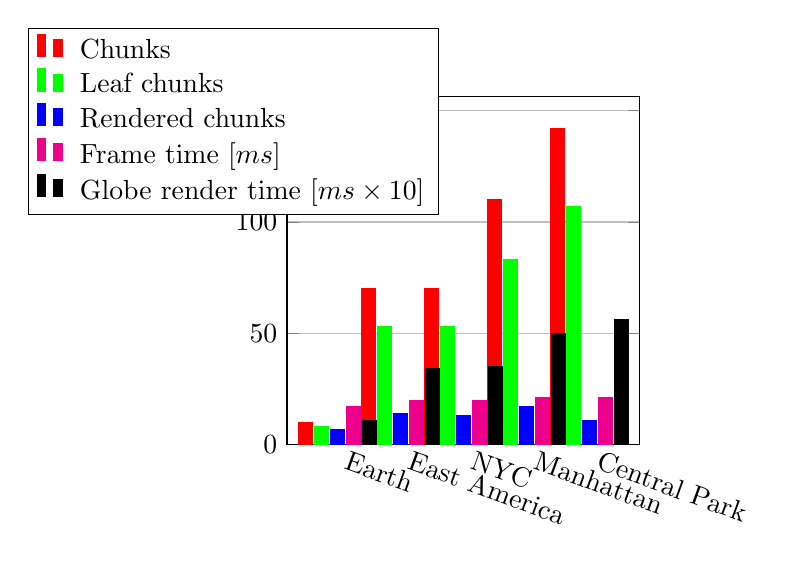
\begin{tikzpicture}
    \begin{axis}[
        width  = 0.5*\textwidth,
        height = 6cm,
        major x tick style = transparent,
        ybar=2*\pgflinewidth,
        bar width=5pt,
        ymajorgrids = true,
        %ylabel = {Number of},
        symbolic x coords={Earth, East America, NYC, Manhattan, Central Park},
        xtick = data,
        scaled y ticks = false,
        enlarge x limits=0.2,
        ymin=0,
        legend cell align=left,
        legend style={
                at={(0.43, 0.66)},
                anchor=south east,
                column sep=1ex
        },
        xticklabel style = {rotate=-20,anchor=west},
    ]

      \addplot[style={red,fill=red,mark=none}]
        coordinates { (Earth, 10) (East America, 70) (NYC, 70) (Manhattan, 110) (Central Park, 142) };

      \addplot[style={green,fill=green,mark=none}]
        coordinates { (Earth, 8) (East America, 53) (NYC, 53) (Manhattan, 83) (Central Park, 107) };
      
      \addplot[style={blue,fill=blue,mark=none}]
        coordinates { (Earth, 7) (East America, 14) (NYC, 13) (Manhattan, 17) (Central Park, 11) };

      \addplot[style={magenta,fill=magenta,mark=none}]
        coordinates { (Earth, 17) (East America, 20) (NYC, 20) (Manhattan, 21) (Central Park, 21) };

      \addplot[style={black,fill=black,mark=none}]
        coordinates { (Earth, 11) (East America, 34) (NYC, 35) (Manhattan, 50) (Central Park, 56) };

      \legend{Chunks, Leaf chunks, Rendered chunks, Frame time $[ms]$, Globe render time $[ms \times 10]$}

    \end{axis}
\end{tikzpicture}
\caption{As the camera descends towards the ground looking straight down, the chunk tree grows but the number of rendered chunks remains relatively constant due to culling.}
\label{fig:topdowngraph1}

\end{figure}

\begin{figure}
    \centering
    	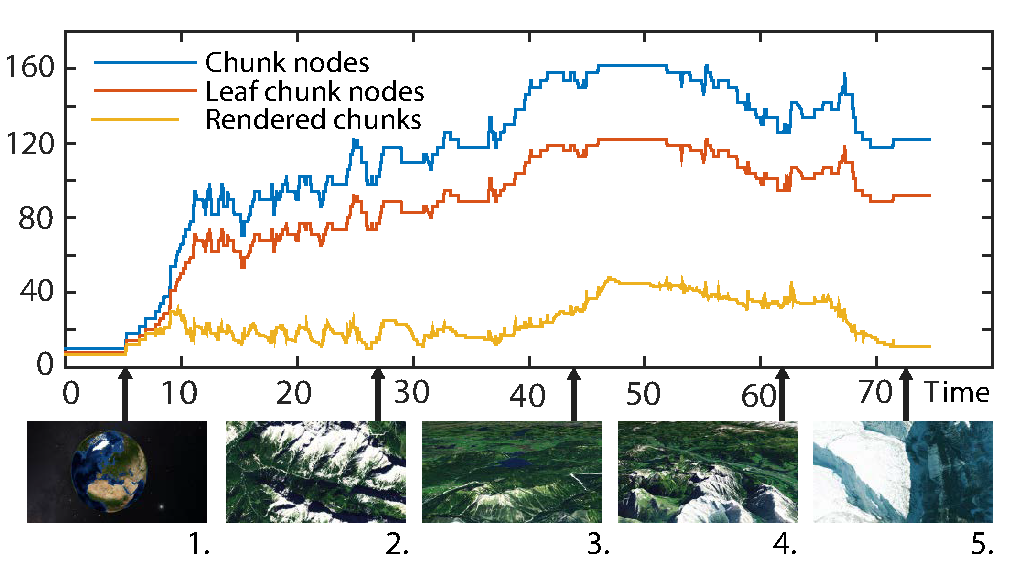
\includegraphics[width=0.5\textwidth]{figures/globebrowsing2.pdf}
    \label{fig:globebrowsing}
\end{figure}
\fi{}


% \begin{enumerate}
% \item Screenshots
% \item Render times
% \item Loading times
% \end{enumerate}

\section{Conclusion and Future Work} \label{sec:conclusion}
In this paper we have presented an application which enables data driven visual browsing of planetary surfaces with dynamic resolution in time and space. The application makes it possible to generate global views as well as virtual terrain fly overs. One of the novel aspects of our work is that it contextualizes the surface data in a seamless astro-visualization environment making it possible to travel form one planet to another, or even visit spacecraft at current locations. The platform used is the OpenSpace~\cite{Bock_2015} software which builds on a dynamic scenegraph and the capability of accurately positioning and visualizing celestial bodies and spacecraft. Another key component presented is the capability to visualize the data acquisition process from the spacecraft perspective, and let the user appreciate the engineering efforts behind complex space exploration missions, while appreciating the origin of the data which drives scientific discovery. Our target use is in science communication and the software has already proven to create engaging immersive experiences in large scale dome theaters. We thus have developed a tool useful both for scientists who want to present their work in a contextualized manner and for the general public who wish to explore the most accurate and open data representation of celestial bodies.

In future work we will further explore the seamless addition of detailed data from surface-based missions such as the Mars rovers. We will also add more data sources such as simulated data of abstract planetary properties. Atmospheric effects is currently in the process of being implemented, as proposed by Elek~\cite{elek2009rendering}. Intuitive and intelligent context dependent navigation models for multi-scale data is also an area with interesting challenges. 


%% if specified like this the section will be committed in review mode
%\acknowledgments{
%The authors wish to thank A, B, C. This work was supported in part by
%a grant from XYZ.}

%\bibliographystyle{abbrv}
\bibliographystyle{abbrv-doi}
%\bibliographystyle{abbrv-doi-narrow}
%\bibliographystyle{abbrv-doi-hyperref}
%\bibliographystyle{abbrv-doi-hyperref-narrow}

\bibliography{references}

\end{document}

